\pdfoutput=1
\pdfcompresslevel=9
\pdfinfo
{
    /Author (Artur Olszak)
    /Title (HyCube protocol documentation)
    /Subject (HyCube protocol documentation)
    /Keywords (HyCube)
}
\documentclass[a4paper,onecolumn,oneside,12pt]{mwrep}

\usepackage{times}
\usepackage[utf8x]{inputenc}
\usepackage[T1]{fontenc}
\usepackage[english]{babel}


\usepackage[toc,page]{appendix}


\usepackage{hhline}


\usepackage{longtable}

\usepackage{tabu}

\usepackage{listings}

\lstdefinestyle{listing1}{
  breaklines=true,
  xleftmargin=\parindent,
  showstringspaces=false,
  basicstyle=\footnotesize\ttfamily,
}

\lstdefinestyle{listing1noindent}{
  breaklines=true,
  resetmargins=true,
  showstringspaces=false,
  basicstyle=\footnotesize\ttfamily,
}

\lstdefinestyle{listing1small}{
  breaklines=true,
  xleftmargin=\parindent,
  showstringspaces=false,
  basicstyle=\scriptsize\ttfamily,
}

\lstdefinestyle{listing1noindentsmall}{
  breaklines=true,
  resetmargins=true,
  showstringspaces=false,
  basicstyle=\scriptsize\ttfamily,
}


\usepackage[table]{xcolor}


\usepackage[normalem]{ulem}


\newcommand{\beq}{\begin{equation}}
\newcommand{\eeq}{\end{equation}}
\newcommand{\refbr}[1]{(\ref{#1})}


\usepackage{graphicx}

\usepackage{amsmath}

\usepackage{amssymb}


\usepackage{float}
\restylefloat*{table}



\usepackage{caption}
\captionsetup{font=footnotesize,labelsep=space,justification=justified,singlelinecheck=false}



\usepackage{multirow}


%\usepackage{morefloats}




%\usepackage{pgfplots}
%\pgfplotsset{compat=newest}



\hyphenpenalty=10000		% nie dziel wyrazów zbyt często
\clubpenalty=10000			% kara za sierotki
\widowpenalty=10000			% nie pozostawiaj wdów
\brokenpenalty=10000		% nie dziel wyrazów między stronami
\exhyphenpenalty=999999		% nie dziel słów z myślnikiem
\righthyphenmin=3			% dziel minimum 3 litery

\tolerance=4500
\pretolerance=250
\hfuzz=1.5pt
\hbadness=1450

\sloppy						% umacnia pozycję prawego marginesu

\setlength{\textwidth}{\paperwidth}
\addtolength{\textwidth}{-2in}
\setlength{\textheight}{\paperheight}
\addtolength{\textheight}{-2in}
\setlength{\marginparwidth}{1in}
\setlength{\oddsidemargin}{0in}
\setlength{\evensidemargin}{0in}

\linespread{1.5}

\begin{document}


\begin{titlepage}	% English title page
	
	\fontseries{b}
	\fontsize{24pt}{18pt}\selectfont
	\emph{HyCube} protocol documentation \\
	
	\fontseries{m}
	\fontsize{16pt}{14pt}\selectfont
	v.1.0.4
	\vspace*{25\baselineskip}
	
	
	\fontsize{14pt}{15pt}\selectfont
	Author: Artur Olszak\\
	\vspace*{1\baselineskip}
	
	
	\begin{flushright}
	\fontsize{10pt}{15pt}\selectfont
	16.10.2016
	\end{flushright}
	
\end{titlepage}


\newpage

\newpage
\pagenumbering{gobble}


This document contains the specification of \emph{HyCube} - a distributed hash table based on a hierarchical hypercube geometry. The presented approach employs a variable multi-dimensional metric adopting the Steinhaus transform. The routing, lookup and search algorithms are presented, as well as DHT resource management algorithms, routing table nodes selection algorithms, self-organization, maintenance and recovery procedures, and enhancements increasing node security and anonymity in the system. The document also specifies the formal protocol, defining the messages exchanged between nodes, their contents, as well as formatting and encoding details.



\newpage

\pagenumbering{arabic}

\setcounter{page}{3}



\tableofcontents



\chapter{System architecture of HyCube - a distributed hash table based on a variable metric}
\label{sec:hycubeArchitecture}

This chapter presents the routing architecture of \emph{HyCube} - a distributed hash table system based on a hierarchical hypercube geometry. Sections \ref{sec:hycubeHierarchicalHypercube} and \ref{sec:hycubeRoutingTables} introduce the hierarchical hypercube concept and describe the structure of routing tables maintained by nodes. Section \ref{sec:routing} presents the basic routing algorithm, and the subsequent sections present various optimizations of the routing algorithm. The optimizations of the basic routing algorithm include the use of a variable routing metric (defining distances between nodes) adopting Steinhaus transform (Section \ref{sec:metric}) - the routing metric is modified by nodes on routes in a way resulting in a very high degree of flexibility in next hop selection (and this a very high level of resilience to node failures), preserving the routing efficiency of the basic algorithm. The concepts presented in this document have been published in \cite{hycubePpam2009} and \cite{hycubeICSReportFeb2013}.





\section{Hierarchical hypercube geometry}
\label{sec:hycubeHierarchicalHypercube}

The routing geometry of \emph{HyCube} is a combination of the tree geometry and the hypercube geometry. It is similar to \emph{Plaxton mesh} \cite{plaxton1}, \cite{plaxton2}, but nodes are also logically located in vertices of a $d$-dimensional hierarchical hypercube. A hierarchical hypercube is a hypercube whose vertices are also (lower level) hypercubes. Vertices of the hypercubes at the lowest level are positions which may be assigned to nodes. 

\begin{figure}
\centering
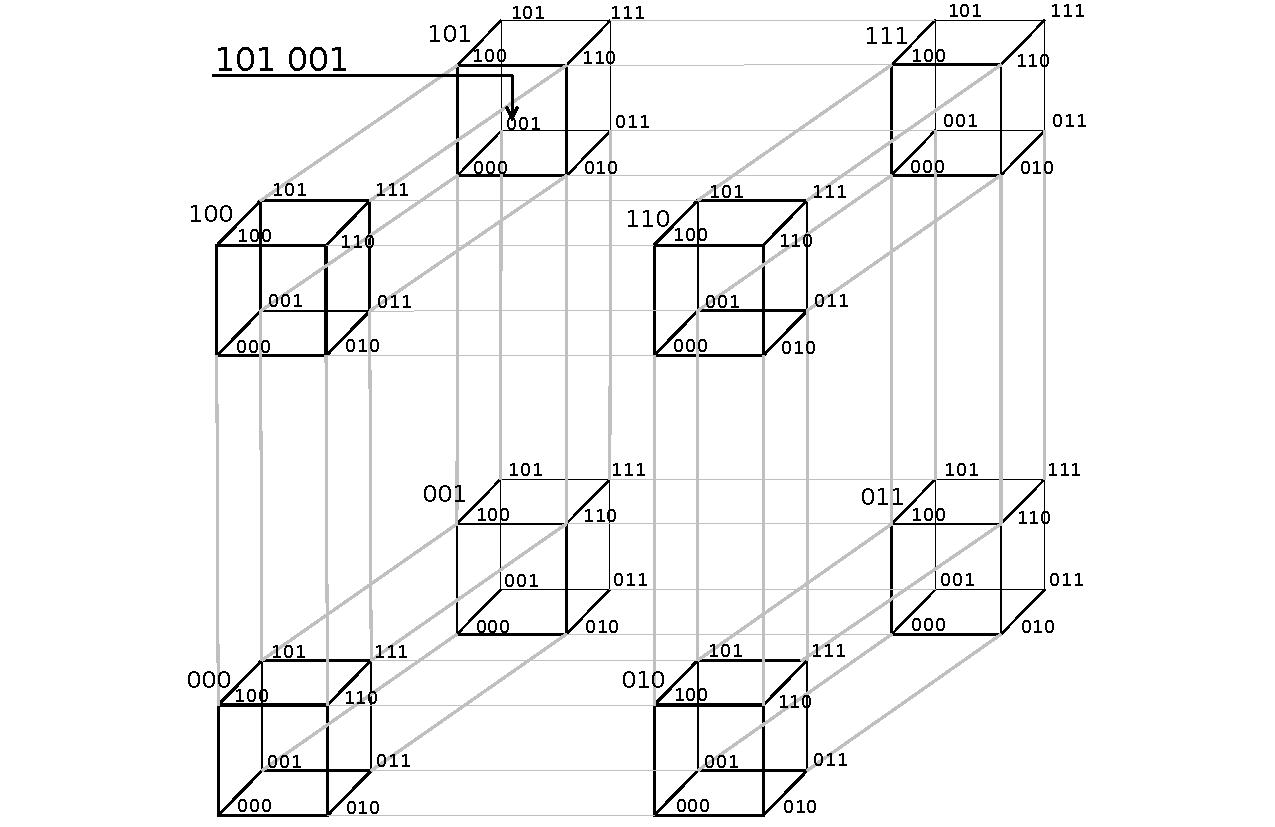
\includegraphics[scale=.6]{img/hh.pdf}
\caption{A hierarchical hypercube (3 dimensions and 2 levels of hierarchy)}
\label{fig:hierarchicalHypercube}
\end{figure}

Figure \ref{fig:hierarchicalHypercube} presents the structure of an exemplary hierarchical hypercube with 3 dimensions and 2 hierarchy levels. Node IDs are determined by their positions - the identifier of a node is a string of $d$-bit groups determining positions of the node in hypercubes at individual levels (starting with the hypercube at the highest level). The position in a hypercube at a particular level is a number built of bits corresponding to the positions of the node in the hypercube in individual dimensions. The length of the identifier equals $d \cdot l$, where $d$ is the number of dimensions, and $l$ is the number of levels.

The hierarchical hypercube and the tree geometries are isomorphic. However, visualizing the structure as a hierarchical hypercube gives an idea of the spatial arrangement of nodes in a $d$-dimensional space - the numbers formed from bits corresponding to individual dimensions relate to the coordinates of the node in these dimensions in the system of coordinates with the center in point $0$. Thus, considering the ID space as a segment of $\mathbb{Z}^d$ space ($\mathbb{Z}$ denotes the set of integer numbers), the distance between nodes may be defined by any metric applicable to $\mathbb{Z}^d$, or $\mathbb{R}^d$ ($\mathbb{R}$ - the set of real numbers) as $\mathbb{Z}$ is a subset of $\mathbb{R}$. However, the geometry of \emph{HyCube} should be seen as a $d$-dimensional torus with the perimeter equal to $2^l$ in each dimension (the set of coordinates in each dimension is treated as on a ring). That means that after the point $2^l-1$, point $0$ is located, and all arithmetic is done modulo $2^l$. This fact is important in determining distances between nodes - in every dimension the distance is determined like on a ring - it is the shorter of the distances in either direction.

In \emph{HyCube}, the default number of dimensions is 4 and the number of levels is 32, resulting in a 128-bit address space (which allows avoiding conflicts of identifiers in majority of applications).



\section{Routing tables}
\label{sec:hycubeRoutingTables}

\subsubsection{Primary routing table.}

The primary routing table has the same structure as in \emph{Plaxton mesh}. It has $l$ levels (the number of hierarchy levels), and, at each level, there are $2^d$ slots ($d$ - the number of dimensions). In the primary routing table of a node $X$, the slot $j$ at level $i$ ($i \geq 0$) contains a reference to a node that is located in the same hypercube at level $i+1$ and in the hypercube corresponding to the number $j$ at level $i$ (lower level). At each level $i>0$, one slot corresponds to the hypercube in which the node $X$ is located - this slot is left empty, as the routing table contains a whole level corresponding to this hypercube.

An exemplary primary routing table for a 2-dimensional hierarchical hypercube with 6 hierarchy levels for node $X$ = 112013 is presented in Table \ref{tab:rt1Example}. For clarity, groups of bits are represented by quaternary digits (base-4 numeral system). The digits in bold represent the sub-hypercube addresses corresponding to routing table slots at individual levels. The underlined digits represent the hypercubes corresponding to the routing table slots matching the hypercubes of node $X$ at individual levels.

\begin{table}
\scriptsize
\begin{center}
%\begin{tabular}{p{2cm}|p{1.3cm}|p{1.3cm}|p{1.3cm}|p{1.3cm}|}
\begin{tabular}{c|c|c|c|c|}
	\hhline{*{1}{~}*{4}{|-}|~|}
																				& \texttt{\textbf{0}}									& \texttt{\textbf{1}}											& \texttt{\textbf{2}}											& \texttt{\textbf{3}}										\\
    \hline
    \multicolumn{1}{|c|}{\texttt{\textbf{Level 5}}}								& \texttt{\underline{\textbf{0}}11033}					& \texttt{-}													& \texttt{\underline{\textbf{2}}31011}							& \texttt{\underline{\textbf{3}}00232}						\\
	\multicolumn{1}{|c|}{\texttt{\textbf{Level 4}}}								& \texttt{\underline{1\textbf{0}}2223}					& \texttt{-}													& \texttt{\underline{1\textbf{2}}1301}							& \texttt{\underline{1\textbf{3}}0001}						\\
	\multicolumn{1}{|c|}{\texttt{\textbf{Level 3}}}								& \texttt{\underline{11\textbf{0}}113}					& \texttt{\underline{11\textbf{1}}201}							& \texttt{-}													& \texttt{\underline{11\textbf{3}}302}						\\
	\multicolumn{1}{|c|}{\texttt{\textbf{Level 2}}}								& \texttt{-}											& \texttt{\underline{112\textbf{1}}01}							& \texttt{\underline{112\textbf{2}}03}							& \texttt{\underline{112\textbf{3}}12}						\\
	\multicolumn{1}{|c|}{\texttt{\textbf{Level 1}}}								& \texttt{\underline{1120\textbf{0}}3}					& \texttt{-}													& \texttt{\underline{1120\textbf{2}}1}							& 															\\
	\multicolumn{1}{|c|}{\texttt{\textbf{Level 0}}}								& 														& 																& 																& \texttt{-}												\\
    \hline
\end{tabular}
\end{center}
\caption{Exemplary primary routing table for node 112013 (for a 2-dimensional hierarchical hypercube with 6 hierarchy levels).}
\label{tab:rt1Example}
\end{table}




\subsubsection{Secondary routing table.}

The secondary routing table of a node $X$ contains nodes from adjacent hypercubes to the hypercube of node $X$ in each dimension, in both directions, at each level. An adjacent hypercube (at any level) is the one whose coordinate in one dimension is greater or smaller by 1 than the coordinate of the same level hypercube of $X$ (modulo $2^l$), and coordinates in all other dimensions are equal to those of $X$. The secondary routing table does not contain nodes in slots at the highest level, as hypercubes corresponding to them are covered by the primary routing table. Also, one of the adjacent hypercubes at each level in each dimension is covered by a primary routing table slot.

The secondary routing table increases the level of flexibility in the next hop selection. If the distance between nodes is defined by a metric in $\mathbb{R}^d$ space, it is very likely that the secondary routing table contains nodes that are closer to any arbitrarily chosen node. Furthermore, it provides additional shortcut references when a message is routed to a node that is close in the $\mathbb{R}^d$ space, but is not close in terms of the \emph{Plaxton mesh} distance. With the use of the primary routing table, routing a message between nodes sharing a short ID prefix would require many steps of traversing the tree structure.

Table \ref{tab:rt2Example} presents an exemplary secondary routing table for node $X$ = 113012 (binary 01'01'11'00'01'10) - for a 2-dimensional hierarchical hypercube with 6 hierarchy levels. For clarity, in this example, the IDs are represented as binary numbers. Addresses of adjacent hypercubes corresponding to the routing table slots are marked in bold, and bits of addresses of adjacent hypercubes corresponding to the particular dimension are underlined - the numbers built of these bits are larger by 1 or smaller by 1 than the numbers formed of the corresponding bits of $X$. All other hypercube address bits (the remaining dimensions) are equal to the corresponding ones of $X$.

\begin{table}
\scriptsize
\begin{center}
%\begin{tabular}{p{1.7cm} p{2.7cm} p{2.7cm} p{2.7cm} p{2.7cm}}
\begin{tabular}{c|c|c|c|c|}
    \hhline{*{1}{~}*{4}{|-}|~|}
														& \multicolumn{2}{c|}{\texttt{\textbf{Dimension 0}}}																																		& \multicolumn{2}{c|}{\texttt{\textbf{Dimension 1}}} 																																							\\
    \hhline{*{1}{~}*{4}{|-}|~|}
														& $\leftarrow$																			& $\rightarrow$																						& $\leftarrow$																						& $\rightarrow$																						\\
	\hline
    \multicolumn{1}{|c|}{\texttt{\textbf{Level 5}}}		& \texttt{-}																			& \texttt{-}																						& \texttt{-}																						& \texttt{-}																						\\
	\multicolumn{1}{|c|}{\texttt{\textbf{Level 4}}}		& \texttt{\textbf{0\underline{1}'0\underline{0}}'01'01'00'11}							& \texttt{\textbf{0\underline{0}'0\underline{0}}'10'01'10'10}										& \texttt{\textbf{\underline{1}1'\underline{1}1}'10'01'00'11}										& \texttt{\textbf{\underline{0}1'\underline{1}1}'00'10'10'01}										\\
	\multicolumn{1}{|c|}{\texttt{\textbf{Level 3}}}		& \texttt{\textbf{0\underline{1}'0\underline{1}'1\underline{0}}'10'01'00}				& \texttt{\textbf{0\underline{0}'0\underline{0}'1\underline{0}}'11'01'01}							& \texttt{\textbf{\underline{0}1'\underline{0}1'\underline{0}1}'11'01'01}							& \texttt{\textbf{\underline{0}1'\underline{1}1'\underline{0}1}'01'00'01}							\\
	\multicolumn{1}{|c|}{\texttt{\textbf{Level 2}}}		& \texttt{\textbf{0\underline{1}'0\underline{1}'1\underline{0}'0\underline{1}}'11'10}	& \texttt{\textbf{0\underline{1}'0\underline{1}'1\underline{1}'0\underline{1}}'01'01}				& \texttt{\textbf{\underline{0}1'\underline{0}1'\underline{0}1'\underline{1}0}'01'10}				& \texttt{\textbf{\underline{0}1'\underline{0}1'\underline{1}1'\underline{1}0}'10'00}				\\
	\multicolumn{1}{|c|}{\texttt{\textbf{Level 1}}}		& 																						& \texttt{\textbf{0\underline{1}'0\underline{1}'1\underline{1}'0\underline{1}'0\underline{0}}'10}	& \texttt{\textbf{\underline{0}1'\underline{0}1'\underline{0}1'\underline{1}0'\underline{1}1}'00}	& \texttt{\textbf{\underline{0}1'\underline{0}1'\underline{1}1'\underline{0}0'\underline{1}1}'10}	\\
	\multicolumn{1}{|c|}{\texttt{\textbf{Level 0}}}		& 																						& 																									& 																									& 																									\\
     \hline
\end{tabular}
\end{center}
\caption{Exemplary secondary routing table for node 113012 (01'01'11'00'01'10) - for a 2-dimensional hierarchical hypercube with 6 hierarchy levels.}
\label{tab:rt2Example}
\end{table}



\subsubsection{Neighborhood set (closest neighbors set).}


In addition to the routing tables described above, nodes maintain sets of closest to them (according to the chosen metric) nodes existing in the system - called \emph{neighborhood sets}. These sets may allow finding a next hop (routing/lookup), decreasing the distance left to the destination, even if there are no appropriate nodes in both routing tables. The closest neighbors sets are expected to increase the probability of delivering messages in the presence of node failures. The neighborhood sets have also very good properties for supporting joining and leaving procedures, as well as maintenance and recovery algorithms, and they help to keep the DHT consistent. Moreover, their existence is crucial for searching closest nodes for a given key, as well as for replicating resources, which will be discussed in detail in Chapters \ref{sec:lookupSearch} and \ref{sec:resourcesManagement}. In \emph{HyCube}, the default size of the neighborhood set is 16.








\section{Basic routing algorithm}
\label{sec:routing}

Let us consider routing a message from node $X$ to node $Y$. Every node $R$ along the route first checks if there is a reference to the destination node in its neighborhood set, in which case, the message is sent directly to that node. Otherwise, the routing tables are searched for an appropriate next hop - the node that shares at least one $d$-bit group longer prefix of ID with $Y$ (than with $R$) or shares the same number of $d$-bit groups of the ID but is closer to $Y$ than $R$ in terms of the chosen routing metric. The routing metric of \emph{HyCube} is discussed in Section \ref{sec:metric}. For the time being, let us assume that routing converges according to the Euclidean metric. The detailed algorithm is presented below:

\begin{enumerate}

\item Initially, the routing algorithm finds the slot in the primary routing table that corresponds to nodes sharing at least one group of $d$ bits longer prefix of ID with $Y$ than with the current node ($R$). In a hierarchical hypercube, this slot corresponds to a hypercube in which the destination node is located, at a lower level than the lowest-level hypercube containing both, the current and the destination node. If for the current node and $Y$, the common prefix length equals $i$, and the next $d$-bit group of the ID of $Y$ equals $j$, $j$-th routing table slot at level $l - 1 - i$ is used. If this slot is not empty, the message is routed to the node found in the slot - increasing the common prefix length with the destination node $Y$ by at least one $d$-bit group.

\item If no node is found in the appropriate primary routing table slot, nodes sharing the same prefix length with $Y$ as with $R$ (in terms of the number of bit groups), but closer to $Y$ in terms of the chosen metric, are also considered - both routing tables and the neighborhood set are checked. From the set of nodes found, the node sharing the longest prefix of the ID with $Y$ (number of $d$-bit groups) is chosen, and, if there are more than one such nodes, the node closest to $Y$ (according to the routing metric) is chosen for the next hop.

\end{enumerate}

The primary routing table supports routing based on extending the ID prefix (in terms of $d$-bit groups) - tree-based routing (\emph{Plaxton mesh}), and the secondary routing table supports finding a closer node in any dimension - such nodes are likely to be closer to the destination node also in terms of the Euclidean metric. Both routing tables and the neighborhood set are used for determining the best possible next hop, to which the message is routed.

It can be shown that the expected route length equals $\lceil\log_{2^d} N\rceil$ hops and, on average, $\lceil\log_{2^d} N\rceil \cdot (2^d-1)$ slots are populated in the primary routing table and $(\lceil\log_{2^d} N\rceil - 1) \cdot d$ in the secondary routing table ($N$ is the number of nodes in the network)\footnote{Based on the assumption that nodes are uniformly distributed in the hierarchical hypercube}.




\subsubsection{Message TTL}

To limit the maximum number of hops for messages, every message contains the TTL information (determining the maximum number of hops) and the number of hops that the message already passed. The TTL value should be decremented, and the number of hops is incremented by every node along the route (including the initiating node) before passing it to the next hop. When the TTL falls below 0, after decrementing, the message should not be routed any further and be dropped.



\subsubsection{Acknowledging message delivery and detecting duplicates}

Optionally, after receiving messages (DATA messages - sent at the application level), depending on configuration, nodes may send acknowledgments (DATA\_ACK messages) confirming receiving of the messages (either directly to the sending node, or routed via the system to the message sender). When the sending node receives the DATA\_ACK message, it knows that the original message was successfully received and processed, and, when no acknowledgment is received (timeout), the node might resend the message (automatic resending may also be configured - up to the defined maximum number of retries). In cases when the acknowledgment mechanism is implemented at the application level (beyond the scope of \emph{HyCube}), the native \emph{HyCube} mechanism may be switched off.

\emph{HyCube} also implements message duplicate detection. In case of receiving a message duplicate, the duplicate is dropped. Message duplicates may be received as a result of incorrect routing or network problems, or an ACK message not being delivered. Duplicates are detected based on the header of the message (the details are specified in Chapter \ref{sec:protocol}).






\section{Number of dimensions versus number of levels}

The address (node identifiers) space should be large enough to prevent potential conflicts of identifiers (existence of two nodes with the same ID). The size of the address space in \emph{HyCube} equals:

\begin{equation}
N_{max} = 2^{d \cdot l}
\end{equation}

\noindent
which means that increasing the number of dimensions or the number of hierarchy levels would increase the number of possible identifiers that nodes may be assigned. However, the number or dimensions and levels of the hierarchical hypercube influences the system characteristics.

Adding additional levels of hierarchy causes the address space to increase, but it also proportionally increases the number of routing table slots that nodes maintain. Moreover, the pessimistic route length would also increase, as in the pessimistic scenario, routing steps correspond to individual routing table levels. Nevertheless, the expected route length remains at the same level, because, on average, similar number of routing table slots would be populated (with high probability the lower-level slots are empty).

Increasing the number of dimensions, on the other hand, has a very strong impact on routing characteristics. Although the routing tables grow sharply with the increase of the number of dimensions, the routing algorithm is more specific in selecting next hops - in each routing step, the common prefix with the destination node ID is increased by a larger number of bits, maintaining the same pessimistic path length and decreasing the average path length. As the base of the logarithm (Equation \ref{equ:expPathLenRT1}) grows exponentially, the expected path length is inversely proportional to the number of dimensions:

\begin{equation}
\label{equ:expPathLenRT1}
\log_{2^d} N = \frac{1}{d} \log_2 N
\end{equation}

\noindent
However, the maintenance cost is significant, as the primary routing table size grows exponentially with the number of dimensions:

\begin{equation}
\log_{2^d} N \cdot (2^d-1) = \frac{\log_{2} N \cdot (2^d-1)}{d}
\end{equation}

At one extreme, when the number of dimensions is equal to the number of identifier bits (1 level of hierarchy), every node would maintain references to all other nodes in the system, and the routing table slots would correspond to all possible values of node identifiers. Increasing the number of dimensions may influence any algorithm used in the distributed hash table and may require adjusting the parameter values for the specified number of dimensions. That is why it is crucial to determine a reasonable value for the number of dimensions that would ensure good routing properties and reasonable sizes of the routing tables, while controlling the identifier length should be done by increasing/decreasing the number of hierarchy levels. Whenever the number of dimensions is changed, it should be verified again that the DHT algorithms parameters still have their optimal values.










\section{Routing table nodes selection}
\label{sec:HyCubeNodeSelection}

The routing table node selection technique used in \emph{HyCube} is a variant of the LNS approach, which, at the same time, provides means to remove failed nodes from routing tables.


\subsubsection{LNS (liveness node selection) in HyCube}
\label{sec:HyCubeNodeSelectionLNS}

\emph{HyCube} uses a variant of LNS which bases the neighbor choice on node liveness information discovered locally, working together with a background process checking node's responsiveness. However, the \emph{HyCube} LNS implementation does not calculate the liveness information based on the node's join and leave times. Every node periodically sends keepalive (PING) messages to all the nodes in its routing tables and updates the stored nodes' liveness values. The value is increased when the node responds to the PING message (sending a PONG message), and is decreased if the keepalive response is not received (timeout). The initial liveness value (new nodes) is defined by the system parameter $L_{init}$, and the values are updated as follows:

\begin{equation}
L = L_{prev} \cdot p + (1-p) \cdot L_{max}
\end{equation}

\noindent
if the keepalive confirmation (PONG message) was received, or:

\begin{equation}
L = L_{prev} \cdot p
\end{equation}

\noindent
when the keepalive fails (no PONG message is returned). $L_{prev}$ is the previous value of liveness, $L$ is the new, updated liveness value, $L_{max}$ and $p$ are system parameters. When $L$ falls below the threshold value $L_{deactivate}$ (system parameter), the node is marked as deactivated and is not used in the routing procedure until $L$ falls below the threshold value $L_{remove}$ (parameter), in which case the node is permanently removed from routing tables, or until $L$ reaches above $L_{deactivate}$ again. Whenever the value of $L$ is below the value of the parameter $L_{replace}$, when possible, the current node in the routing table slot is replaced by a new node, whose value $L$ is then given the initial value $L_{init}$. The value of $L$ for any node removed from the routing table should however be stored by nodes for some time to prevent replacing new nodes that temporarily fall below $L_{replace}$ with nodes that were permanently unresponsive. The values $0 < p < 1$ (update coefficient), $L_{deactivate}$, $L_{replace}$ and $L_{remove}$ determine the sensitivity of the algorithm, and $L_{max}$ defines the maximum value of $L$. This technique provides a good way to keep long-living responsive nodes in routing tables and eliminate failed or overloaded nodes that are not able to handle requests. Reasonable values of $p$, $L_{deactivate}$, $L_{replace}$ and $L_{remove}$ should be chosen to prevent the algorithm from removing nodes from routing tables in case of temporary delays in sending responses by nodes, but still, to be able to efficiently remove failed nodes. If $L_{max} = 2$, the values of $L_{init} = 1.5$, $p = 0.5$, $L_{deactivate} = 1$, $L_{replace} = 0.5$ and $L_{remove} = 0.05$ are good defaults as they allow avoiding failed paths due to temporary nodes' unresponsiveness, at the same time allowing unresponsive nodes to be replaced by new nodes. Using these default values would cause deactivating nodes after a single failed keep-alive, however, not replacing/removing them immediately. The parameter values (as well as the keep alive interval) may be fine-tuned depending on the system characteristics. The flexibility in next hop selection guaranteed by \emph{HyCube} ensures that no significant increase in failed paths rate, nor the average path length, is observed even if large portions of nodes temporarily do not respond to keep-alive messages and are deactivated.




\subsubsection{\emph{HyCube} mixed mode node selection}

The LNS technique described above allows replacing a routing table node only when its value of $L$ drops below $L_{replace}$ (or when $L$ reaches $L_{remove}$, in which case the node is removed). In some cases, however, it would be desirable to take another criterion (or criteria) into account, like for example proximity or any application specific measure. To achieve that, the condition $L < L_{replace}$ may be relaxed, and the neighbor selection could be based on a function measuring both factors - the liveness and the second factor (algorithm-specific). The liveness fulfillment factor may be defined as follows:

\begin{equation}
	Fact_{L} = \left|\frac{L - L_{replace}}{L_{replace}}\right|^{e_L} \cdot \mathop{\mathrm{sgn}}(L - L_{replace})
\end{equation}

\noindent
where the exponent $e_L$ determines the exponential growth of $Fact_{L}$ depending on the difference $L - L_{replace}$. Depending on the algorithm, this factor may be used to calculate overall criteria fulfillment at a node level, improvement of the criteria fulfillment for a new node, relative to current node(s), or may be used in calculating the quality function value for a set of nodes (for example for the neighborhood set). An exemplary neighbor selection criterion at a node level might be a weighted sum of two factors:

\begin{equation}
	Q = \alpha \cdot Fact_{L} + \beta \cdot Fact_{X}
\end{equation}

\noindent
where $Fact_{X}$ may be any neighbor selection algorithm specific function.







\section{Prefix mismatch heuristic}
\label{sec:pmh}

In the final part of a route, when the message is already relatively close to the destination node, the routing algorithm may omit some nodes that are close to the destination, but do not share the same long or longer prefix of ID with the destination node than with the current node. This phenomenon becomes more significant when a multidimensional metric is used. That is why, like in \cite{pastry}, \emph{HyCube} uses a heuristic switching to routing based only on the distance left, when a message is already in vicinity of the destination. Nodes should therefore be able to determine how close the message is to the destination in relation to the density of nodes in the space. In \emph{HyCube}, before choosing the next hop, each node checks if the distance to the destination is shorter than the average distance to the nodes in the neighborhood set multiplied by the factor $\lambda$: 

\begin{equation}
d_{dest} < \mathop{\mathrm{avg}}(d_{neigh}) \cdot \lambda
\end{equation}

\noindent
If this condition is satisfied, all further nodes on the route are chosen based only on their distance to the destination node - they might not share the same long or longer prefix of the identifier. All nodes from both routing tables and the neighborhood set are checked and the closest node is chosen for the next hop.

The prefix mismatch heuristic may be also enabled, when no next hop is found with routing based on extending the common prefix length with the destination node. This behavior may be configured by changing a system parameter value. In many cases, the number of neighborhood set nodes matching the destination is much larger if the selection is based only on the distance. Obeying the prefix condition is a much stronger constraint on the next hops, and may cause more failed paths, especially in the presence of many node failures. Thus, although the path length might increase, by default, \emph{HyCube} switches to routing based only on the distance left whenever no next hop is found. To maintain routing convergence, the prefix mismatch heuristic is followed by all subsequent nodes along the path.

The greater is the value of $\lambda$, the longer parts of routes will be determined based only on the distance left. The value should be large enough to ensure high probability of message delivery. However, too large values of $\lambda$ could cause an increase in path lengths. The performed simulations indicated that the value $\lambda = 1.5$ ensures good static resilience, maintaining the path lengths at a low level.





\section{Routing metric}
\label{sec:metric}

In DHT systems, distances between pairs of nodes are defined by a certain metric, and the routing converges according to this metric. The choice of the metric has a great impact on the average route length and the probability of message delivery. \emph{HyCube} uses a variable multi-dimensional metric adopting the Steinhaus transform, described in this section. It was confirmed during simulations that such an approach allows reaching a very high level of resilience to node failures and short pessimistic and average routing/lookup paths.




\subsection{Steinhaus transform}
\label{sec:steinhaus}

In \cite{nearNeighSearchMetrSpDim} and \cite{geomCutsMetrics}, the authors present the Steinhaus transform. The terminology comes from the fact that this distance was used in biological problems for the study of biotopes \cite{certDistSetsCorrDistOfFunc}. The theorem presented says that if $D$ is a metric on a set $X$, $D'$ is also a metric on $X$ for any $a \in X$, where:

\begin{equation}
\label{equ:steinhaus}
D'(x,y) = \frac{2D(x,y)}{D(x,a) + D(y,a) + D(x,y)}
\end{equation}

The default base metric used in \emph{HyCube} ($D$ in the equation above) is the Euclidean metric. Applying a metric with the Steinhaus transform to every route, setting the value of $a$ to the ID of the source node, causes the next hops to be chosen in such a way that they are closer to the destination node and more distant from the source node. Such an approach increases the expected number of neighborhood set nodes to which messages may be routed in each routing step - although some closer nodes (according to metric $D$) might be considered more distant when the Steinhaus transform is applied, it allows sending messages using more roundabout routes, while still being convergent to the destination node.

One important remark should be made regarding the Steinhaus transform. In the case when $x = y = a$, Equation \ref{equ:steinhaus} does not have a value (division by zero). Therefore, the value of the distance should be considered 0 if $x = y$, regardless of the value of $a$.



\subsection{Variable metric adopting Steinhaus transform}
\label{sec:varSteinhaus}

The use of the Steinhaus transform yields very good routing parameters and very high resilience to node failures for networks containing relatively few nodes. However, for networks containing much more nodes (denser), in final parts of routes, the addend $D(x,a)$ of the denominator in Equation \ref{equ:steinhaus} (where $x$ is the current node), has less influence on the value of the distance as its changes in individual steps are very small compared to the value of the entire denominator. Thus, the more nodes in the network, the lesser is the influence of the Steinhaus transform on routing. However, a certain modification can be introduced - a variable metric adopting the Steinhaus transform, where point $a$ would be changed by intermediate nodes along routes. The value of $a$ would initially be set to the source node $ID$, and subsequent nodes, before choosing the next hops, would check whether they are closer (in terms of the Euclidean metric) to the destination than the current point $a$. In such a case, point $a$ would be updated - would be given the value of the current node. Such a way of changing point $a$ ensures that the routing is convergent to the destination (there will be no cycles on routes) and yields a very high level of flexibility in the next hop selection along the whole route, regardless of the network size. It is easy to notice that whenever the Steinhaus point has the value of the current node ID, messages may be passed to any other node, decreasing the Steinhaus distance left to the destination. With great probability the node closest to the destination in terms of the Euclidean metric is chosen. It may however not be a node that is closer (Euclidean) to the destination. Nevertheless, in such a case, the subsequent next hop selections would be more restrictive and converge to the destination faster. The expected route length is still proportional to $\sqrt[d]{N}$, and, owing to the increase in the flexibility in the next hop selection, the resilience to node failures reached is very high.

It should be noted that whenever the Steinhaus point is equal to any of the node IDs between which the distance is measured, the distance value equals 1, regardless of the second argument value:

\begin{equation}
D'(x,y)\bigg|_{a=x} = \frac{2D(x,y)}{D(x,x) + D(y,x) + D(x,y)} = 1
\end{equation}

\begin{equation}
D'(x,y)\bigg|_{a=y} = \frac{2D(x,y)}{D(x,y) + D(y,y) + D(x,y)} = 1
\end{equation}

\noindent
When calculating distances from multiple nodes to the destination node, if the Steinhaus point is given the value of the destination node ID, it is impossible to differentiate the nodes, as all the distances are then equal to 1. The routing algorithm is not exposed to such a situation - the Steinhaus point value would be equal to the destination point only when the destination is already reached. However, any other algorithm using Steinhaus distances, modifying the Steinhaus point, should take that fact into account (e.g. search algorithm, described in Sec. \ref{sec:lookupSearch}).



To limit the average route length increase caused by employing the variable Steinhaus metric, one more modification was introduced - the Steinhaus transform should be used only when the prefix mismatch heuristic is already applied. The use of the Steinhaus transform is the most important when the message is already in the proximity of the destination node, and the probability of finding the next hop in the neighborhood set drops sharply with the use of the Euclidean metric. If the Steinhaus transform is used only when the prefix mismatch heuristic is applied, it is enabled when the message gets close to the destination, or when no next hop is found (which would also enable the prefix mismatch heuristic, allowing the Steinhaus transform to be used). Such a modification decreases the average path length, preventing messages from being routed to more distant areas (according to the Euclidean metric) in initial steps, when the average hop distances are much larger. Despite a significant decrease of the average path length, the modification did not cause any static resilience decrease.






\section{Euclidean distance versus Steinhaus distance - re-routing using regular metric}
\label{sec:euclideanAfterSteinhaus}

The final steps of routing with the use of a metric with the Steinhaus transform applied may cause a message to be sent to a node that is more distant from the destination than it would be if the Steinhaus transform was not applied. Therefore, when, at some point, a node on a route cannot find the next hop in its routing tables and neighborhood set, it is possible that the route is ended in a point (node) that is not the closest one to the destination in terms of the Euclidean metric. For some applications, if the destination node itself cannot be reached, it is crucial to reach the closest possible node. Thus, \emph{HyCube} introduces one more modification - when a message cannot be routed by a node, the node tries to route it again, based only on the Euclidean distance left to the destination. All consecutive next hops after that should be chosen in the same way. Such an approach will cause that, in the case the message is dropped, a relatively close node to the destination is reached. From the experiments (for a network containing 10'000 nodes, with 50\% failed nodes, routing using only neighborhood sets), it appears that applying this phase in routing allows messages to be sent to a closer node in about 80\% cases. Furthermore, this additional phase of routing also increases the resilience of the system to node failures.

There is, however, one drawback of such an approach - the failed path lengths (undelivered messages) may possibly increase due to re-routing with another metric after the next hop is not found. Nevertheless, messages usually get relatively close to the destination node, and, in most cases, only a small number of additional hops (if any) are performed.






\section {Uniform distribution of neighborhood set nodes}
\label{sec:uniformNSDistribution}

The neighborhood set should provide possibility to route messages regardless of the direction in which the destination node is located. Therefore, it is important that nodes in neighborhood sets be uniformly distributed in terms of directions. There might be a scenario where some nodes would have more closest neighbors in one direction and no or very few neighbors in other directions. In such a case, the nodes would not be able to route messages in all directions (using neighborhood sets). The issue becomes more important in the presence of node failures, when the number of matching next hops should be as large as possible. In a multi-dimensional space, it is not trivial to ensure uniform distribution of the closest neighbors set, ensuring that certain subset of these nodes would match any potential direction (message destination). Uniform distribution of nodes in terms of directions may be defined in a variety of ways, and many different algorithms may be employed to maximize this uniformity. Both, proximity and even distribution, should be considered, because ensuring uniform distribution of nodes in respect of directions may cause some more distant nodes to be included in neighborhood sets and pass over some closer nodes. The key is to maintain the good properties of neighborhood sets (as being the closest existing nodes), and to make these good properties valid regardless of the direction.

\emph{HyCube} adopts a simple technique for ensuring uniform distribution of neighborhood set nodes in respect of directions. The technique splits the space into fragments (orthants\footnote{An \emph{orthant} is the generalization (in $d$-dimensional Euclidean space) of a quadrant (2-dimensional space)} of the system of coordinates with the center at the address of the node whose neighborhood set is considered) and attempts to ensure that in each orthant, the number of nodes is the same. Within individual orthants, nodes are chosen based on their distances. Such a solution is very simple, efficient and does not require much computational overhead. 





\section{Hypercube-aware next hop selection}

When the routing algorithm cannot find a node sharing a longer ID prefix with the destination node than with the current node, a node sharing the same long prefix, but closer to the destination according to the chosen metric is selected as the next hop. When the message is routed within a hypercube corresponding to the common prefix length according to the distance only, it is completely independent of the hypercube hierarchy at lower levels. It is however possible to introduce one more criterion in next hop selection. If the message was routed to a node sharing the largest possible number of common bits in the first different digit (group of $d$ bits), this would be the node in the closest possible hypercube at a lower level. If there were more than one such nodes, the next hop would be then chosen by the remaining distance (among the nodes with the same number of common bits in the first different digit). Such an approach increases the probability of finding the next hop sharing longer prefix (in terms of entire bit groups) by the next node(s) on the path - with the support of secondary routing tables.






\section{Routing table slots overlapping}
\label{sec:rtOverlapping}

Hypercubes corresponding to slots of primary and secondary routing tables may contain nodes that are covered by a slot at a lower level in the secondary routing table. If multiple different routing table slots contain the same node, when the node fails, all these slots become unusable. That is why, ideally, the routing tables should contain references to different nodes for all such overlapping hypercubes.

To overcome the overlapping problem, for the secondary routing table, it is enough to consider a node as a candidate for a matching routing table slot only if the corresponding adjacent hypercube is the lowest-level hypercube containing that node (for individual dimensions and directions). That would ensure that no secondary routing table slot would contain nodes that are located in overlapping lower-level adjacent hypercubes.

As far as the primary routing table slots are concerned, it may also be easily verified whether a certain node is covered by a lower-level secondary routing table slot (let us denote by $Y$ its identifier, and by $X$ the ID of the node whose routing table is being considered). $X$ and $Y$ are in adjacent hypercubes at levels $l - 1 - j$ to $l - 1 - i$ if and only if all $k<i$ first digits ($d$-bit groups) of $X$ and $Y$ are equal, and $i$-th to $j$-th digits differ on one (the same for all these digits) bit - this bit corresponds to the dimension in which the two hypercubes are adjacent. $l$ is the number of levels, and $d$ is the number of dimensions of the hierarchical hypercube. If $l - 1 - j$ is smaller than the corresponding primary routing table level of $Y$, $l_{RT1}$, that means that $Y$ is located in an adjacent hypercube at a lower level than $l_{RT1}$ and is thus covered by a lower-level secondary routing table slot. There might also be a case that $Y$ is not in an adjacent hypercube in any dimension at any level - if the first different digit ($d$-bit group) of $X$ and $Y$ differs on more than one bit.

This modification, however, should not be applied to the neighborhood set, because the neighborhood set is crucial for maintaining high resilience and should always contain the closest nodes (as discussed in the previous sections). Thus, the neighborhood set might contain some nodes that are also included in routing tables. Furthermore, when considering a candidate for routing tables, no check whether the node is in the neighborhood set should be performed. The neighborhood set is continuously updated, and such a check might very soon be ``out-of-date'', while still having left the routing table slot empty. Therefore, due to its properties, the neighborhood set should be built independently from the routing tables.










% ex: set tabstop=4 shiftwidth=4 softtabstop=4 noexpandtab fileformat=unix filetype=tex encoding=utf-8 fileencodings= fenc= spelllang=pl,en spell:



\chapter{Lookup and search procedures}
\label{sec:lookupSearch}

The previous chapter concentrated on the geometry and the routing algorithm of \emph{HyCube}. From the DHT perspective, two other algorithms are also of a great importance - lookup and search. Instead of routing a message, in many cases, it is more adequate for a node to find a node or nodes that are the closest ones in the system to a given key (node ID) and communicate with these nodes directly. Because lookup and search algorithms are performed by multiple nodes, the whole lookup/search process will be referred to as lookup/search procedures. Lookup is a procedure performed by a node that results in finding the node closest to a given ID, while search results in finding a requested number of closest nodes to the given key in the system. During the lookup/search procedure, the initiating node communicates with other nodes in the system, retrieving information about their neighbors. Using the references returned, the searching node makes decisions which nodes should be contacted next, until the closest nodes are found. No message is routed further, and, in each step, the decision which nodes should be contacted next is made locally.

In both, lookup and search procedures, the initiating node may require the requested nodes to return multiple references to nodes closest to the specified key. The routing tables are searched exactly as described in Section \ref{sec:routing}, but the next hop selection finds the requested number of best next hops, according to the same criteria. If multiple references are supposed to be returned by the next hop selection algorithm, the prefix mismatch heuristic (Section \ref{sec:pmh}) or falling back to Euclidean routing (Section \ref{sec:euclideanAfterSteinhaus}) is applied only when no nodes are found at all. Often, the next hop selection algorithm might not be able to find as many nodes fulfilling the next hop criteria as requested. In such cases, if at least one node is found, the next hop selection is considered successful, and the node/nodes found are returned to the requestor.



\section{Lookup procedure}

In the node lookup procedure, as opposed to routing, next hop selection is made by the initiating node. Nodes receiving the lookup request do not route the message, but they send back (to the initiating node) a reference to a node or nodes that are the best next hop candidates. However, the decisions regarding the next node selection are made locally. This is sometimes referred to as iterative routing, as opposed to recursive routing. To ensure that the procedure is convergent to the lookup node, next hops must satisfy the same conditions as in the routing procedure, i.e. they must share a longer prefix with the destination node than with the previous node or share the same prefix length but be closer to the lookup node than the current node. The metric used is the same as the one used in routing, and the prefix mismatch heuristic also applies whenever a node close enough is reached. When the lookup node is found, it may then be contacted directly, and application-specific operations may be performed. Although node lookup requires more network traffic, and the overall lookup latency is greater (the number of messages exchanged is at least doubled), the main advantage of such an approach is the possibility of returning and sending the lookup request to another node whenever any node requested does not return closer references. This reduces the risk of a route failure due to any single node not being able to route the message, and additionally makes it possible to find the lookup node using more roundabout paths. The node lookup procedure is initiated with three parameters:

\begin{itemize}
	\renewcommand{\labelitemi}{$\bullet$}
	\item $key$ - the ID of the lookup node
	\item $\beta$ - the maximum number of nodes returned by intermediate nodes
	\item $\gamma$ - the number of temporary nodes stored during the lookup
\end{itemize}

\smallskip
\noindent
During the whole lookup, the initiating node maintains a set $\Gamma$ containing $\gamma$ closest (Euclidean) nodes found so far. The lookup procedure consists of two phases:

\begin{enumerate}

\item Initially, $\Gamma$ is filled with at most $\gamma$ closest nodes (to the lookup node ID) from local routing tables and the neighborhood set (variable Steinhaus metric), and the initial lookup request is sent to the closest node in $\Gamma$. After receiving a response from the requested node (max. $\beta$ references), $\Gamma$ is updated so that it includes $\gamma$ closest nodes from the nodes currently stored in $\Gamma$ and the returned nodes, and the next request is sent to the node returned. If, however, no node is returned, the next request is sent to the closest node in $\Gamma$ that has not been yet requested.
For every node stored in $\Gamma$, virtual route information is maintained - the Steinhaus point and flags indicating whether the prefix mismatch heuristic has already been enabled for this virtual route and whether the Steinhaus transform has been switched off (no closer nodes found with the use of Steinhaus transform). Initially, for all nodes found in local routing tables, the Steinhaus point is set to the ID of the initiating node, and the prefix mismatch heuristic flag is set based on the analysis of the local neighborhood set. These values are included in every lookup request, and the requested nodes should take these parameters into account during next hop selection (local closest nodes search). Every requested node, during the next hop selection, updates the Steinhaus point for the virtual route if it is closer to the destination (Euclidean) than the current Steinhaus point, determines (based on its neighborhood set) whether it is close enough to the lookup node to enable the prefix mismatch heuristic (which then remains enabled for this virtual route), and whether the Steinhaus transform should not be applied any more (no closer nodes found with the use of Steinhaus transform). The updated parameter values are sent back to the requestor within the lookup response message. The procedure continues until the lookup node reference is returned, or until no new nodes are returned.

\smallskip
\item When the lookup node is not found (the lookup request has been sent to all the nodes in $\Gamma$ and no closer nodes were returned), the lookup procedure is repeated on the current set $\Gamma$, but is based on the Euclidean metric (no Steinhaus transform), and the prefix mismatch heuristic is enabled (like in the routing procedure). Because for certain nodes (virtual routes) in $\Gamma$, the prefix mismatch heuristic might have already been enabled, there is no need of sending additional requests to them. The closest node found after this phase is considered to be the closest node in the DHT.

\end{enumerate}

The initial lookup (local), in addition to the closest nodes found in the local routing tables, should also consider adding the initiating node (itself) to $\Gamma$, as it may be one of the closest nodes to $key$. If the initiating node ID is one of the $\gamma$ closest nodes found locally, it should be placed in $\Gamma$. Furthermore, the initiating node ID may be returned by any intermediate node (for any virtual route after changing the metric to Euclidean, the initiator node ID may become closer than the current node). No additional local search is however required in the first phase, as it was already performed initially. However, when this node ID (self) is still in $\Gamma$ after switching to the second phase (Euclidean metric and prefix mismatch heuristic in use) a local search should be performed with the prefix mismatch heuristic enabled and based only on the Euclidean distances. Otherwise, some potential references to closer nodes (stored locally) might be omitted.

When $\beta = 1$ and $\gamma = 1$, the node lookup procedure creates one virtual route that is exactly the same as if the message was routed. By increasing $\beta$ and $\gamma$, in case of failures, the procedure is capable of returning and creating alternative routes, and allows sidestepping inconsistent fragments of the connection graph.




\section{Search procedure}
\label{sec:search}

The purpose of the search procedure is locating $k$ nearest nodes to a given key (identifier) in terms of the Euclidean metric. Search is a basic functionality of a distributed hash table - it is used for storing and retrieving resources and when a new node joins the network. The closest nodes search, like the node lookup procedure, is managed locally by the initiator, which sends search requests to nodes and analyzes the responses. The decisions to which nodes next requests should be sent, are made by the initiating node. The search procedure is initiated with the following parameters:

\begin{itemize}
	\renewcommand{\labelitemi}{$\bullet$}
	\item $key$ - the ID for which $k$ nearest nodes should be found
	\item $k$ - the number of closest nodes to be found
	\item $\alpha$ - the number of closest nodes to which search requests are sent (parallelism factor)
	\item $\beta$ - the maximum number of nodes returned by intermediate nodes ($\beta \geq k$)
	\item $\gamma$ - the number of temporary nodes used during the search ($\gamma \geq k; \gamma \geq \alpha$)
	\item $ITN$ - ``ignore target node'' - determines whether the set of $k$ nodes should contain the exact match (the node with the identifier equal to the requested $key$) or not
\end{itemize}

\smallskip
\noindent
During the whole search, the initiating node maintains a set $\Gamma$ containing at most $\gamma$ nodes, closest (in terms of the Euclidean metric) to $key$ found so far. The initiating node sends search requests to the closest nodes and processes the responses received. After receiving a response from any node (to which a search request has been sent), the set $\Gamma$ is updated so that it contains at most $\gamma$ nodes closest to $key$ (Euclidean). The search procedure consists of two phases:

\begin{enumerate}

\item In the first phase, the set $\Gamma$ is initially filled with maximum $\gamma$ nodes from local routing tables and the neighborhood set, that are the closest to $key$ (variable Steinhaus metric). In the consecutive steps, the initiating node sends the search request to nodes in $\Gamma$ which have not yet been requested and are within $\alpha$ closest nodes to $key$ found so far. After receiving a search request, the receiving node looks for at most $\beta$ nodes closest to $key$ in its routing tables and neighborhood set. As opposed to the lookup procedure, the closest $\beta$ nodes returned in the search procedure do not have to satisfy the prefix condition, and do not have to be closer to $key$ than the current node. However, the routing tables are searched for $\beta$ nodes sharing the longest prefix with $key$, and among the nodes sharing the same prefix length, the choice is made based on the distance to $key$ (with the use of the variable Steinhaus metric if the prefix mismatch heuristic is already switched on). Upon receiving a search response, the initiating node updates $\Gamma$ with the nodes returned, so that it contains the closest nodes to $key$ from the nodes currently stored in $\Gamma$ and the newly returned nodes.
For every node in $\Gamma$, the current Steinhaus point is stored, as well as a flag indicating whether the prefix mismatch heuristic has already been applied for finding the node. These values are included in search requests sent to nodes, and the local searches are performed based on these parameters. These parameters may be modified by the nodes processing search requests (updating Steinhaus point if the current node ID is closer to $key$ than the current Steinhaus point, and enabling the prefix mismatch heuristic based on the local neighborhood set), and the updated values are included in the search responses. The first search phase finishes when none of $\alpha$ currently closest to $key$ nodes returns any node closer to $key$ than the most distant node in $\Gamma$ - all $\alpha$ closest nodes in $\Gamma$ have been already requested and returned the responses (or the requests timed out).

\smallskip
\item The second search phase is a repetition of the first phase, however, requests are sent to all the nodes in $\Gamma$, the prefix mismatch heuristic is enabled, and only the Euclidean metric (no Steinhaus transform) is used in local searches. The search is finished when none of the nodes in $\Gamma$ returns any node closer to $key$ than the most distant node in $\Gamma$. The result of the procedure is $k$ closest nodes to $key$ from the set $\Gamma$.

\end{enumerate}

The second search phase (without the use of the Steinhaus transform) is extremely important, because during the search, nodes are allowed to return also more distant nodes to the $key$ than themselves. There would never be a situation in which no node is found in the routing tables (unless the routing tables are empty, in which case switching to Euclidean routing would as well return no nodes). Thus, the routing tables would never be searched for nodes closest in terms of the Euclidean metric (finding no nodes is the condition for switching off the Steinhaus transform), which could lead to omitting some nodes that are close to $key$.

The initial search (local), in addition to the closest nodes found in the local routing tables, should also consider adding the initiating node itself to $\Gamma$ (if the initiating node ID is one of the $\gamma$ closest nodes found locally), as it might be one of the closest nodes to $key$ in the system. Furthermore, a reference to the initiating node may be returned by any requested node, in which case, no additional local search is required in the first search phase, as it was already performed initially. However, when this node ID (self) is still in $\Gamma$ after switching to the second phase (Euclidean metric and prefix mismatch heuristic in use), a local search should be performed again with the prefix mismatch heuristic enabled and based only on the Euclidean distances. Otherwise, some potential references to closer nodes (stored locally) might be omitted.

The value of $\gamma$ should be at least equal to $k$. However, it may be greater than $k$ to allow more roundabout search paths. Especially, for small values of $k$, such roundabout paths are important so that the procedure finds also the nodes that are located in the hierarchical hypercube on the opposite side of the point $key$ than the initiating node.

Whenever a local search (next hop selection) is performed by a certain node for the $key$ equal to its own identifier (which would update the value of the Steinhaus point to the value of $key$ - it would be the closest point reached so far), the search should be continued without the use of the Steinhaus transform (all virtual routes starting from this node). If the value of the Steinhaus point is equal to the $key$ (destination), as described in Section \ref{sec:varSteinhaus}, $D'(x,y) = \frac{2D(x,y)}{D(x,a) + D(y,a) + D(x,y)} = \frac{2D(x,y)}{D(x,y) + D(y,y) + D(x,y)} = 1$, regardless of the distance $D(x, y)$. This fact would make it impossible to differentiate nodes based on the distance to $key$. Such a scenario would never happen during the lookup procedure, as finding the exact match would immediately return it. However, it is very important when considering the search procedure.

If the parameter $ITN$ is set to \emph{true}, the value of this parameter is included in every request message, and all local searches (next hop selections) should skip the exact match. This parameter is useful when a node performs a search for closest nodes to its own identifier. In such a case, returning a reference to itself would make no sense. There is also no need to re-check local routing tables after switching to the second search phase, because when the distance equals 0, the initial local search would be performed with the prefix mismatch heuristic enabled anyway, and the Steinhaus metric would not be applied.

As opposed to the lookup procedure, in the search procedure, the initial values of the Steinhaus points (for initial nodes in $\Gamma$ found locally) are not set to the initiating node ID, but to the IDs of the initial search nodes themselves. If the initiating node is closer to $key$ than the requested node (at one extreme equal to $key$, in which case the Steinhaus transform would never be applied), the influence of using the Steinhaus transform could possibly be reduced.







% ex: set tabstop=4 shiftwidth=4 softtabstop=4 noexpandtab fileformat=unix filetype=tex encoding=utf-8 fileencodings= fenc= spelllang=pl,en spell:




\chapter{Self-organization}
\label{sec:selfOrganization}

This chapter describes the algorithms emplyed by \emph{HyCube} for joining/leaving the network, as well as maintenance and recovery processes, maintaining good routing properties under dynamically changing conditions. The algorithms are based on nodes exchanging information about references stored in routing tables and neighborhood sets. When a node receives a notification about existence of some other peer or receives references maintained by some other node (requested for example in the recovery or joining process, or generated by the notifying node itself), it should analyze the node and check if the reference should be stored in the routing tables or the neighborhood set. Every node is analyzed as a candidate to the neighborhood set and appropriate routing table slots. 
For the primary routing table, this is the slot at the level calculated based on the common prefix length with the node ($l - 1 - commonPrefixLength$, $l$ - the number of hierarchy levels) at the position equal to the first different digit (group of $d$ bits, $d$ - the number of dimensions).
For the secondary routing table, the slot corresponds to the lowest-level hypercube containing the analyzed node, adjacent to the hypercube of the analyzing node. A simple check may be performed to verify this condition: nodes $X$ and $Y$ are in adjacent hypercubes at levels $l - 1 - j$ to $l - 1 - i$ if and only if $i$ first digits ($d$-bit groups) of $X$ and $Y$ are equal, and $i$-th to $j$-th digits (numbered starting from 0) differ on one (the same for all these digits) bit - this bit corresponds to the dimension in which the two hypercubes are adjacent, and only the slot at the lowest level should be considered (to prevent placing the same nodes in overlapping routing table slots at different levels). Furthermore, depending on settings, additional rules described in Section \ref{sec:rtOverlapping} may apply to prevent storing nodes in the primary routing table slots overlapping with the lower-level secondary routing table slots.
For selecting nodes within individual routing table slots and within the neighborhood set, the algorithms described in Sections \ref{sec:HyCubeNodeSelection} and \ref{sec:uniformNSDistribution} apply.




\section{Maintenance and recovery}

Maintenance is a process of ensuring good system properties that takes place continuously (ensuring the relevance of routing tables, updating information about neighbors). The maintenance mechanism used in \emph{HyCube} is directly connected with the routing table neighbor selection (described in detail in Section \ref{sec:HyCubeNodeSelectionLNS}). Every node periodically sends keepalive messages to all the nodes in its routing tables, and, depending on whether the keepalive response is received or not, the node's liveness value is updated. Based on the liveness value, the routing table reference may be skipped in the next hop selection (to avoid failed paths), may be replaced, or removed from the routing tables.

Recovery is a process of repairing the network topology and propagating necessary information over the network on account of a topology change (new nodes joining/leaving the system), topology breakdown (node failures) or attacks. The recovery technique, employed by \emph{HyCube}, is a periodic procedure, run every specified time interval (parameter value). The value of the interval should be adjusted depending on the DHT nature. The higher is the level of churn, the recovery should be run more often, while if the system has a very stable nature, this interval might be larger. The recovery algorithm in \emph{HyCube} proceeds in two phases:

\begin{enumerate}

\item In the first phase, the node sends a recovery request to all nodes in its routing tables, which it turn return their routing tables to the requesting node. Upon receiving the responses, the requesting node processes the references returned and updates its routing tables and neighborhood set.

\item In the second recovery step, the node performing the recovery sends a notification (NOTIFY message) about its existence to all nodes in its neighborhood set and routing tables (immediately after sending the recovery requests). The notification is also sent to the routing tables nodes to spread the information about the node to more distant parts of the hypercube. However, to limit the overhead, the maximum number of the routing table nodes to which notification is sent should be limited - the message would be sent to certain maximum number of nodes (random selection from all routing table nodes).

\end{enumerate}

Because such an approach may lead to exchanging a large number of messages and also increase processing overhead at the node level, neighborhood set recovery - a variant of the recovery was introduced. Nodes performing the neighborhood set recovery send the recovery requests only to nodes in their neighborhood sets, which dramatically decreases the network traffic and processing overhead. In addition to the recovery interval, \emph{HyCube} allows defining the recovery plan - determining a sequence of recovery variants (for individual recovery runs, successive recovery types from the recovery plan are performed - following a cyclical pattern). Full recovery has better properties in terms of keeping the routing tables up-to-date. However, especially for larger networks, the overhead is significantly larger. Although there might be situations in which the neighborhood set is completely corrupt, and sending recovery requests to the routing table nodes would return much more nodes, usually it is sufficient to repeat the neighborhood set recovery instead. Therefore, the neighborhood set recovery is the default recovery method used in \emph{HyCube}.

To spread the information about the node in an even greater degree, it is possible to send a notification also to every node to which a reference is returned in recovery responses. However, this approach proved to generate enormous network traffic, as well as very high nodes' processing overhead. Performed simulations proved that notifying all neighborhood set nodes and 16 random routing table nodes during every recovery does not significantly increase the overhead, and, if the recovery procedure is run frequently enough, it is sufficient to properly propagate the information about the node's existence. Furthermore, depending on configuration, nodes may process the recovery request messages as notifications (analyze the sender as a routing table candidate), in which case, a notification message does not have to be later sent to the nodes to which the recovery requests were sent.




\section{Joining the system (connecting to the DHT)}

When a new node joins the existing DHT, it should have knowledge about any node already connected to the system. \emph{HyCube} implements two different approaches for joining the system. One of them is based on routing a JOIN message through the system to the node closest to the new node's ID, and the routing tables are formed by the references returned by intermediate nodes along the path (including also themselves), as well as the closest node. The second method is based on searching for the nodes closest to the new node's ID, which form initial routing tables for a new node. The routing approach requires much less overhead - a smaller number of messages are exchanged. However the search method is not vulnerable to any single node possibly causing the join message to be dropped. This section presents both join techniques.



\subsection{``Route-join'' procedure}

The route-join procedure is based on the joining mechanism presented in \cite{pastry}. To initiate the route-join procedure, the joining node should send a ``join'' request (JOIN message) to any node already participating in the system. The message is routed to the closest possible node to the joining node's ID (however, omitting the exact match, as the message would be possibly routed back to the joining node). All intermediate nodes send back (directly to the joining node) JOIN\_REPLY messages that contain all references stored by them in their routing tables. Every node returned is analyzed by the joining node and its routing tables are updated based on the criteria described in Sections \ref{sec:HyCubeNodeSelection} and \ref{sec:uniformNSDistribution}. As the message gets closer to the new node ID, references returned are more likely to be good candidates for the neighborhood set. Furthermore, as the common prefix length with the joining node ID increases, more and more routing table slots correspond to the same hypercubes as the one of the joining node, so more and more references returned by the intermediate nodes might be also used for building the routing tables. For that reason, it is a good idea to disable the prefix mismatch heuristic for JOIN messages (the behavior is configured by a system parameter).




\subsection{``Search-join'' procedure}

In the search-join procedure, the joining node initially retrieves all references from routing tables from a known node connected to the system. The references returned are used to perform a search (Section \ref{sec:search}) for the closest nodes to the joining node ID with certain values of parameters $\alpha$, $\beta$, $\gamma$: $\alpha_{join}$, $\beta_{join}$ and $\gamma_{join}$ (system parameters), and the $ITN$ (ignore target node) parameter set to \emph{true}. The value of $k$ is not important, because all nodes returned by intermediate nodes are processed (updating the routing tables). Initially, the set $\Gamma$ is filled with $\gamma$ closest (Euclidean) nodes retrieved in the initial phase - from the bootstrap node. Afterwards, the search procedure proceeds as described in Section \ref{sec:search}.

Because the node performing the search is the node whose identifier is being looked for, to allow the use of the Steinhaus transform, the initial values of Steinhaus points should not be set to the joining node ID (Euclidean metric would be then used for local next hop selections), but should be given the values of IDs of the initial nodes themselves (only for the initial nodes returned by the bootstrap nodes - for any nodes added to $\Gamma$ later, the Steinhaus point is updated based on the information contained in the response message that contained the node reference).










\section{Leaving the system (disconnecting from the DHT)}

The maintenance and recovery mechanisms should be able to maintain connection graph consistency and keep routing tables of nodes up-to-date, ensuring good routing and searching properties. However, these algorithms have certain ``inertia'' and react with a certain delay. A simple solution to overcome this problem is sending the leave information (LEAVE message) to all neighbors in the leaving node's neighborhood set. Such LEAVE messages should contain the list of neighborhood set nodes of the leaving node, and the nodes receiving it should remove references to the LEAVE sender from the routing tables and the neighborhood set, and process all the nodes included in the message to immediately fill the lost routing table or/and neighborhood references.









% ex: set tabstop=4 shiftwidth=4 softtabstop=4 noexpandtab fileformat=unix filetype=tex encoding=utf-8 fileencodings= fenc= spelllang=pl,en spell:




\chapter{Managing resources}
\label{sec:resourcesManagement}

This chapter focuses on the resource storage architecture of \emph{HyCube} and describes individual DHT operations. Possible operations on the resources in \emph{HyCube} include inserting resources to the DHT (PUT) and retrieving resources (GET). Additionally, \emph{HyCube} supports refreshing resources (REFRESH) - updating resource expiration times, removing resources from the DHT (DELETE), and resource replication among nodes. In \emph{HyCube}, the nature of resources, as well as the way of calculating the resource key depends at the application - \emph{HyCube} provides generic support for any resource type. The key (hash) is expected to be within the node identifier space - $(d \cdot l)$-bit number ($d$ - the number of dimensions, $l$ - the number of levels of the hierarchical hypercube), and the node responsible for resources with the hash value $key$ is the closest node to $key$ (Euclidean metric) among all nodes existing in the system. However, to increase the availability and provide load balancing, the resource may be replicated to other nodes (certain number of closest nodes to $key$).

There are two main approaches for storing resources - one is based on storing the actual resources (for example files) by the DHT nodes to which the resource keys are mapped, while the second approach is based on storing pointers by the DHT nodes - the information where individual resources are stored (for example from which nodes particular files may be downloaded). The technique adopted by \emph{HyCube} is universal and the choice which approach is used is made at the application level. The resource entries in \emph{HyCube} (stored by nodes) consist of a resource descriptor (metadata) and resource data. However, the data may be empty, and the pointer to the actual data might be stored within the resource descriptor, or within the data field. The resource descriptor consists of a certain number of key-value pairs (both keys and values are text strings). There are four predefined keys for resource descriptors:

\pagebreak

\begin{itemize}
	\renewcommand{\labelitemi}{$\bullet$}
	\item \emph{\textbf{resourceId}}	- should be a unique identifier of the resource, allowing to unambiguously distinguish it from any other resource
	\item \emph{\textbf{resourceUrl}}	- determines the location of the resource, allowing to unambiguously locate the resource copy among possible multiple copies/instances of the same resource (having the same value of resourceId)
	\item \emph{\textbf{resourceName}}	- the name of the resource
	\item \emph{\textbf{resourceType}}	- resource type (possible values, as well as the way the type is used, are application-specific)
\end{itemize}

Specifying values for \emph{resourceId} and \emph{resourceUrl} is mandatory, because these values are used by the resource management algorithms (storing, refreshing, getting, deleting and replication). A resource key may theoretically be the same for multiple different resources (usually it is the result of a hash function on the resource name or content), and \emph{resourceId} is essential to unambiguously distinguish the resources. If the resource entries stored in the DHT are used only as references to nodes storing actual resources, \emph{resourceUrl} value should make it possible to uniquely locate the resource copy that the entry points. Depending on a system parameter value, nodes may store multiple copies of the same resource if the \emph{resourceUrl} values are different.

In addition to four predefined resource descriptor keys, at the application level, additional keys may be defined. The resource metadata might then be used to apply additional query criteria on the resources returned by nodes - only resources matching all criteria specified in queries (GET) would be returned to the requesting node. The criteria might also be used when deleting resources from the DHT.

The following sections describe the operations supported by \emph{HyCube} DHT. The discussion focuses on operations on resource entries and assumes that they contain the resource data. If the data is, in fact, located somewhere else, and resource entries are only pointers, it is assumed that the actual data insertion, retrieval and deletion is handled by the external application, beyond the scope of \emph{HyCube}.




\section{Storing resources in the DHT}

The PUT operation allows a node to store a resource in the distributed hash table. A node initiating a PUT operation routes a PUT message containing the resource descriptor (and data) specifying the resource key as the message recipient. The message is routed to the closest node to the specified key (until no further routing is possible), which saves the resource in its local storage and sends the status of the operation (PUT\_REPLY message containing the information whether the resource was saved in the node's local storage or not) directly to the requesting node. Before storing the resource, the closest node checks whether it is one of the $k_{store}$ closest nodes to the specified key ($k_{store}$ is the system parameter). Based on this check, the node decides whether the resource should be accepted or not. The check is made based on analyzing the local neighborhood set. For that purpose, a local estimation of the network ``density'' $\rho$ (the author's definition) is calculated as follows:

\begin{equation}
\rho = \frac{\sum_{i=0}^{t} \rho_i}{t+1}
\end{equation}

\noindent
where $\rho_i$ is defined as follows:

\begin{equation}
\rho_i = \frac{\left|\{N \in NS : dist(N) \leq dist(N_i)\}\right|}{dist(N_i)^d}
\end{equation}

\noindent
where $NS$ is the neighborhood set, $dist(N)$ denotes the distance to node $N$, $d$ is the number of dimensions of the hierarchical hypercube, and $t \in [0, |NS|-1]$ is the node index (in the neighborhood set ordered ascending by distances) calculated as follows:

\begin{equation}
t = \max \big(0, \mathop{\mathrm{round}}(\varphi \cdot |NS|) - 1 \big)
\end{equation}

\noindent
where $\varphi \in (0,1]$ is a system parameter - the quantile function threshold, determining what number of closest neighborhood set nodes should be taken into account for calculating the density. Each density $\rho_i$ represents the number of nodes in a unit $d$-sphere calculated based on $(i+1)$-th node (the value $dist(N_i)^d$ in the denominator is proportional to the volume ($d$-dimensional volume) of a unit $d$-sphere, so $\rho_i$ is proportional to the real local density). $\rho$ is the average density - based on all $t+1$ nodes. Calculating the average value makes the density estimation less vulnerable to fluctuations of single node distances.

Based on $\rho$, it is possible to estimate the number of nodes in the system in a $d$-sphere of any given radius $r$:

\begin{equation}
n = \rho \cdot r^d
\end{equation}

\noindent
Thus, the estimated radius of the $d$-sphere containing $k$ closest nodes to any given key may be calculated as:

\begin{equation}
r_k = \left(\frac{k}{\rho}\right)^{\frac{1}{d}}
\end{equation}

Having calculated $r_k$ for $k = k_{store}$, it is possible to estimate whether the node is one of the $k_{store}$ closest nodes to any given key - the node should check if the distance to the key is less than or equal to $r_k$. However, such en estimation might not be accurate enough. The radius used for the density calculation is the minimum radius covering the number of nodes considered (distance to $N_i$), which may cause nodes to incorrectly estimate the density, resulting in the number of nodes accepting resources being smaller than $k_{store}$. Taking this problem into account, it is necessary to scale the estimated value $r_k$, and the node should rather check whether the following condition is met:

\begin{equation}
dist(key) \leq r_k \cdot \xi
\end{equation}

\noindent
$\xi$ is the system parameter - estimated distance coefficient. The value should be adjusted for the chosen value of $\varphi$. The higher is the value of this parameter, the more nodes will accept resources, considering themselves as one of $k_{store}$ closest nodes to the resource key. The value should be large enough to ensure that resources will be accepted by at least $k_{store}$ nodes in the system, regardless of their key. Because for certain nodes, the locally calculated density may be smaller than the average density, for certain keys, more nodes than $k_{store}$ could potentially accept the resource. This is however not a serious issue, meaning that the resource will be more likely to be accepted in less dense areas, which would have positive impact on replication under churn (replication is discussed in Section \ref{sec:replication}).

When the neighborhood set nodes selection forces the diversity of directions in which the nodes are located, the most distant neighbors might not reflect the real closest existing nodes (omitting some close nodes). In such a case the real density could be higher than estimated. Performed simulations showed that, in such a case, the numbers of nodes accepting resources start growing rapidly for $\varphi > 0.5$. Because forcing uniform distribution of neighborhood set nodes is the default behavior in \emph{HyCube}, $\varphi$ should be given a value smaller than 1 to achieve better accuracy (skipping the most distant nodes). However, too small values of $\varphi$ would cause the density to be calculated taking only a very small number of nodes into account. Although the density estimation may skip some close nodes even for smaller values of $\varphi$, the performed simulations indicated that the value $\varphi=0.5$ provides good and relatively stable density estimation (relatively small variance of the numbers of accepting nodes).

The simulation results indicated that, for $\varphi=0.5$, the values of $\xi \geq 1.1$ allow resources to be accepted by at least $k_{store}$ nodes for great majority of randomly generated keys. For values $\xi \geq 1.2$, almost for all tests, at least 8 nodes accepted the resources. $\xi$ should be given a higher value if the nodes should be accepted by more than $k_{store}$ nodes, for example to force accepting resources by each of $k_{store}$ closest nodes to the key (which is a different condition than accepting resources by any $k_{store}$ nodes\footnote{Because the local density may be different in the proximity of the estimating node, and the resource key, certain more distant nodes may accept the resource, while some close nodes may reject the resource.}). It may, however, cause resources to be potentially accepted by a larger number of nodes. When resources are required to be accepted by a certain number of closest nodes (by all of the closest nodes) with high probability, it may also be ensured by increasing the value of $k_{store}$, leaving the value $\xi$ equal to 1.1 or 1.2, which would also cause the resources to be accepted by more nodes, at the same time, increasing the probability of accepting resources by the closest nodes to the resource keys. The values of these parameters should be adjusted to actual needs, depending on the application.

When a node accepts a resource, it stores the resource in its local storage, making it accessible for other nodes to retrieve (GET). Because potentially, there might be many resource entries with the same key, but not representing the same resource (different \emph{resourceId}), such resources are considered separate entities and are stored separately. Furthermore, it is possible for a node (depending on the value of a system parameter) to store multiple resources with the same \emph{resourceId}, but having different values of \emph{resourceUrl}. Such resource entries represent the same resource located physically in different locations. The maximum number of resource entries stored for any \emph{resourceId} is determined by the value of another system parameter.

When resources are being stored by nodes, they are assigned expiration times (the resource validity time is determined by a system parameter). After the expiration time elapses for any resource, the resource is deleted from node's local storage.



\section{Refreshing resources in the DHT}

As described in the previous section, every resource is given an expiration time, and the resource entry contains the last refresh time. After the expiration time (\emph{refreshTime} + \emph{expirationTime}), the resource is deleted from the storing node's local storage. To prevent deleting resources, the node placing the resource in the DHT may send a REFRESH\_PUT message to the node storing the resource, which would renew its refresh time. The new refresh time is sent within the refresh message. However, if the refresh time received is greater than the current local time, the new refresh time is given the value of the current local time. To avoid problems caused by two nodes potentially located in different time zones, the refresh time should always be converted to the UTC (Coordinated Universal Time). The REFRESH\_PUT message is routed towards the resource key, and when no next hop is found (closest node was reached), a check is made whether the resource with the specified \emph{resourceId} and \emph{resourceUrl} is present in the local storage and whether the node is one of the $k_{store}$ closest nodes to the resource key. If both conditions are met, the node updates the refresh time for the resource entry and sends a REFRESH\_PUT\_REPLY message directly to the requesting node. The REFRESH\_PUT\_REPLY contains the status of the operation. If at least one of the checks fails, a negative response is sent.

This mechanism is supposed to prevent maintaining resources inserted to the DHT when they are no longer current. Nodes publishing resources in the DHT should therefore periodically refresh their validity time, and the refresh interval should be smaller than the resource expiration time.




\section{Retrieving resources from the DHT}

In order to retrieve (GET) resources from the DHT, a node sends a GET message containing the requested key and additional criteria, specifying the requested key as the message recipient. Depending on the value of the request parameter \emph{GetFromClosest}, the message is either routed to the node closest to the resource key, which searches its local storage for the resources according to the specified criteria, or the resource(s) are returned by the first node on the route that is able to return the resource(s). The returning node sends back (directly) a GET\_REPLY message containing the results, or an empty result, depending whether the resources were found or not. If \emph{GetFromClosest} equals \emph{false} (the resource is supposed to be returned by the first node on the route storing it), every node on the route (including the initiating node itself) first makes a check, whether the node is one of $k_{store}$ closest nodes to the resource key, and whether the resource requested is stored in the local storage. If both conditions are met, the result is immediately returned directly to the requesting node. Otherwise, the node tries to route the message. If, however, the message cannot be routed because no next hop is found in the routing tables (the closest node is reached), the node returns the results found locally (if any), even it is not one of the $k_{store}$ closest nodes to the resource key. This method of retrieving resources yields very good properties in terms of load balancing if the resource is replicated to multiple nodes (Section \ref{sec:replication}). When the message reaches one of the $k_{store}$ closest nodes, this node is likely to contain all published copies of the resource, while if the route is broken before one of the nodes maintaining the resource (considering itself as one of the $k_{store}$ closest nodes) is reached, this node may return only partial result or not return anything at all (resources might have been stored in that node in the past, and, in some cases, resources may be replicated to more than $k_{store}$ nodes).

Every GET request, in addition to the resource key, contains additional resource search criteria (key-value pairs). The criteria key set should be a subset of the resource descriptor key set. Before returning the GET result, nodes filter out the resources, and only resources matching the criteria are returned (matching resource descriptor values for all the keys specified in the criteria).






\section{Resource removal from the DHT}

In certain applications, it would be desirable to allow nodes to remove (DELETE) resources that have been earlier inserted into the distributed hash table. \emph{HyCube} provides such a possibility. A node willing to delete a resource should send a DELETE message addressed to that node (or to the resource key, in which case the message would be routed to the node closest to the resource key), specifying the exact criteria for deletion - key-value pairs (the key set should be a subset of the resource descriptor key set: \emph{resourceId}, \emph{resourceUrl}, \ldots). The resource entry should be deleted only when all key-value pairs specified within the criteria match those of the resource entry descriptor. For instance, a node might decide to delete a resource copy published by itself, while still leaving other copies of the resource accessible. In this case, the node would specify the \emph{resourceId} and \emph{resourceUrl}, which unambiguously identifies that particular instance of the resource. Every node processing a DELETE message is supposed to send a DELETE\_REPLY message directly to the requestor, containing the status of the operation (\emph{true} is the resource was deleted, \emph{false} otherwise).

When a resource is removed from one node's local storage, it may still be accessible through other nodes, and may be again inserted to the node that removed it through the replication mechanism. That is why the resource being removed should be deleted from all nodes storing the resource at the same time. It is however never guaranteed that the resource is entirely deleted from the DHT, as it is difficult to track to which nodes the resource was replicated. All resources are however assigned the expiration time (mentioned earlier), which causes resources to be deleted after certain amount of time if they are not refreshed. This mechanism is able to eventually remove outdated resources from the DHT completely.






\section{Storage access control}

By default, in \emph{HyCube}, it is possible to perform PUT, REFRESH\_PUT, GET and DELETE operations on any resource by any node. In many cases, this behavior might not be desirable. The design of \emph{HyCube} allows introducing an additional (application defined) component that would control which operations are allowed and which are not, based on the resource descriptor and the node performing the operation. For example, such a mechanism might be enabled to allow REFRESH\_PUT and DELETE operations to be performed only by the nodes that originally put the resource in the DHT. Such a check could be based for example on the \emph{resourceUrl} value. Another example could be limiting access for resources for certain nodes based on the resource metadata.




%\section{Exact versus routed resource operations}
\section{Routing requests vs sending requests directly to nodes}

As described in the previous sections, PUT, REFRESH\_PUT, GET and DELETE messages are routed towards the resource key, and the responses are returned directly to the requesting node. However, another approach may be taken if the request should be sent to a certain exact node (known to the requesting node). In such a case, this exact node's ID should be set as the recipient of the message and the message should be sent directly to the recipient. The message would then not be routed further, even if it is not the closest node to the resource key. Specifying the exact recipient for resource operation messages allows placing resources in multiple nodes, updating the refresh time (REFRESH) for resources stored in multiple nodes, and retrieving the resources from several nodes at a time. Usually, to increase resource availability, the resource is stored in several nodes - the closest nodes to the resource key. Moreover, as already mentioned, the DELETE operation would successfully remove a resource from the DHT only if the resource is removed from all the nodes storing it. To determine the set of closest nodes, the search procedure may be performed, and the messages may then be sent directly to the nodes found. Depending on the application, other techniques may be employed - for instance, if the resource should be put to only one node (for example allocation of subtasks in a distributed computing system), a node lookup might be used to find the node closest to a certain identifier.

In majority of applications, the resources are stored by multiple nodes, and the PUT operation should usually be preceded by the search locating the closest nodes, to which the resources are then inserted. However, retrieving the resources from the DHT, in most cases, may be done more efficiently, without the use of the search procedure. In the routing approach (towards the resource key), it is possible to limit the number of messages exchanged between nodes to the minimum, finding the resource with high probability in the closest node to the resource key. If additionally, the value of the option \emph{GetFromClosest} is set to \emph{false}, the check is made by all nodes on the route, increasing the probability of finding the resource requested. Furthermore, such a way of retrieving resources would provide simple, but effective load balancing - the first node containing the resource would be different depending on the path (direction from which the request comes).







\section{Resource replication and load balancing}
\label{sec:replication}

It was already mentioned that, to increase availability of resources, they may me replicated to multiple nodes. In \emph{HyCube}, resources are replicated among a certain number of nodes (let us denote this number by $k_{rep}$) that are the closest ones to the resource keys ($k_{rep}$ is a system parameter). However, in dynamic systems, the set of $k_{rep}$ closest nodes may change very quickly, making resources difficult to locate. At one extreme, all nodes responsible for some resource key may leave the system, making the resources unavailable. Therefore, it is crucial that the resources get constantly replicated among $k_{rep}$ currently closest nodes. $k_{rep}$ may be larger than $k_{store}$, but in this case, some nodes may not return the replica when receiving a GET message (with the \emph{GetFromClosest} option set to \emph{false}) - instead they would route the message further towards the resource key. 

The replication procedure is run periodically by all nodes. Every node sends information about all resources it maintains to all the nodes in its neighborhood set (REPLICATE messages). To keep the message sizes at reasonable levels, the resources stored for different keys should be sent in separate REPLICATE messages. The number of nodes to which the replication information is sent may be limited to a certain maximum number of nodes by setting the value of the system parameter \emph{maxReplicationNSNodesNum}, in which case the REPLICATE messages will be sent only to \emph{maxReplicationNSNodesNum} closest nodes in the neighborhood set. However, to allow resources to be replicated towards all directions in the Euclidean space, the value of this parameter should not be too low. The replication information contains only the resource descriptors (metadata) and the last resource refresh time. Upon receiving a REPLICATE message, for every replicated resource, the receiving node should check if it is one of the $k_{rep}$ closest nodes to the resource key. If the node is one of the closest nodes, for each resource corresponding to that key, the node should check if it maintains this resource in its local storage. If the resource is already stored (\emph{resourceId} and \emph{resourceUrl} are compared), the refresh time of the resource should be updated (if the refresh time for the resource in the replication message is greater than the local refresh time). If the resource is, however, not stored in the local storage, the node should perform the GET operation (GET messages routed towards the resource key, the value of \emph{GetFromClosest} flag used in replication is set by a system parameter), and, upon receiving the GET\_REPLY, insert the resource to its local storage, setting the refresh time to the one received in the REPLICATE message. However, if the refresh time received is greater than the current local time, the refresh time is set to the current time.

The replication mechanism of \emph{HyCube}, in addition to increasing resource availability, also provides load balancing for most popular resources. \emph{HyCube} is designed to realize this approach by allowing an external (application-specific) module, implementing an appropriate interface, to be registered - a replication spread manager, which may analyze all PUT, REFRESH\_PUT, GET and DELETE operations and calculate the replication spread factor $\psi$ for each resource stored. Based on $\psi$, the node performing the replication calculates to how many nodes the resource should be replicated:

\begin{equation}
k_{rep} = \psi \cdot k_{rep}
\end{equation}

\noindent
where $k_{bal}$ is the default number of replication nodes. The value of $k_{bal}$ for every resource is included in the REPLICATE messages sent to nodes. The nodes receiving replication information, accept the replicas only when they determine that they are within $k_{bal}$ closest nodes to the resource key. For more popular resources, the replication spread manager may increase the value of $\psi$, which would cause the resource to be replicated to more nodes. When combined with retrieving (getting) resources with \emph{GetFromClosest} option set to \emph{false}, such a replication mechanism provides very good load balancing - in a multidimensional space, the increase of the replication radius would cause more nodes handling GET requests coming from different directions. As already mentioned, the value of $k_{rep}$ (and thus $k_{bal}$) may be greater than the system parameter $k_{store}$. However, in this case, some nodes, although accepting the replica, would not return the resource when receiving a GET message with the \emph{GetFromClosest} option set to \emph{false}. The implementation of the replication spread manager is application-dependent and is beyond the scope of \emph{HyCube}. The default implementation returns the value $\psi = 1$ for every resource.

One more remark should be made regarding replication and updating refresh times for resources. Whenever there is a time difference between any two nodes, the refresh time sent within a REPLICATE message may be inadequate when the message is received by another node. That could potentially cause the refresh time to be automatically increased just by the replication process, which is not a desired behavior. However, the new refresh time assigned to resources is always the smaller of the two values - the refresh time received and the current local time, meaning that the refresh time will never be increased by exchanging REPLICATE messages to a larger value than the current local time. The refresh time may also be increased as a result of receiving a REFRESH\_PUT message, when a larger refresh time value is specified by the refreshing node. Although there is also a possibility that the refreshing node's time is shifted (relatively to the node receiving the refresh request), the refresh time will never be set to a greater value than the receiving node's local time. Thus, the only potentially problematic situation may occur when both, the refreshing and the refreshed node have their local clocks going faster. In such a case, the refreshed node would potentially send a wrong refresh time in replicate messages (potentially far in future). However, as other nodes would then set the refresh time to their current local time value, and the replicating node (the one with the clock going faster) would stop replicating the resource after it is outdated according to its local time, the excess storing time at the whole DHT level would, at one extreme, be equal to the resource expiration time (the worst case), and the resource would then be considered outdated and removed by all other nodes.

The replication mechanism employed by \emph{HyCube} is able to maintain replica availability in the presence of many node failures, as well as under high rates of churn. Although in such situations, it may happen that certain resources are replicated to more nodes than needed, this anomaly would be only temporary - the excess replicas would be removed after their expiration time (the resources stored by the excess nodes would not be refreshed).

Although replicating resources is performed every certain time interval, the algorithm does not introduce much overhead, because only a small number of REPLICATE messages are exchanged, and nodes physically transfer the resources only when it is needed.








% ex: set tabstop=4 shiftwidth=4 softtabstop=4 noexpandtab fileformat=unix filetype=tex encoding=utf-8 fileencodings= fenc= spelllang=pl,en spell:




\chapter{Security and privacy}
\label{sec:security}

The following sections discuss the security enhancements employed by \emph{HyCube}, which are essential elements of real peer-to-peer systems, as well as the privacy features that provide anonymous request-response communication, maintaining the identities of both communicating parties secret. Section \ref{sec:secureRouting} presents two routing security enhancements - introducing the secure routing tables concept and randomized next hop selection. Section \ref{sec:accessControlAuthentication} discusses access control and authentication mechanisms - it is explained how application-specific access control and authentication mechanisms may be incorporated into the \emph{HyCube} architecture. Section \ref{sec:congestionControl} describes the congestion control mechanism employed by \emph{HyCube}, preventing overloading nodes with processing large numbers of messages, at the same time limiting nodes' vulnerability to DoS/DDoS attacks. Section \ref{sec:privacy} discusses privacy issues - data encryption and anonymity. The section presents the registered and anonymous routes concept, allowing the communicating parties to retain their identities secret.



\section{Secure routing}
\label{sec:secureRouting}

\subsubsection{Secure routing tables}

In \cite{secrouting1}, the authors propose secure routing tables - additional constrained routing tables maintained by nodes, which may be used when messages are not delivered with the use of regular routing tables. The constrained routing tables are created based on some strong constraint on the set of node IDs that can fill each slot of the routing table. The constraint should be strong enough to make it difficult to be manipulated by potential attackers. The authors suggest that each entry in the constrained routing table be the closest to the desired point $P$ in the ID space. In the extension of \emph{Pastry} DHT, they define point $P$ as follows: for a routing table of a node with identifier $X$, the slot $j$ at level $i$ (the routing table slot may contain nodes with IDs that share the first $i$ digits with $X$ and have value $j$ in the $i+1$-th digit), $P$ shares the first $i$ digits with $X$, it has the value $j$ in the $i+1$-th digit, and it has the same values of remaining digits as $X$. Nodes closest to meeting this condition (the remaining digits closest to the ones of $X$) would be chosen for the secure routing tables. This approach is a good heuristic for limiting attacks based on propagating false information about possible routing table candidates, because the probability of any node's ID meeting that condition for large number of peers is very low.

The above strategy (with modifications) has been adopted by \emph{HyCube}. For each routing table slot (primary or secondary routing table), the point $P$ is defined as follows: it has the first $i$ digits equal to the address of the hypercube corresponding to the routing table slot and remaining digits equal to those of $X$. Such a formulation is equivalent to the original definition but expressed using the hierarchical hypercube terminology and extending the definition to cover also the secondary routing table. However, the process of calculating the constraint for routing table nodes in \emph{HyCube} is different. In the original solution, the distance from the point $P$ to the ID of the routing table slot candidate is minimized. In \emph{HyCube}, the value being minimized is the distance between $P$ and the point being the result of the XOR operation on the candidate's ID and a certain secret key, maintained by each node. This secret key may be randomly re-generated after analyzing every $n_{change}$ candidates ($n_{change}$ is a system parameter). Additionally, to avoid replacing the constrained routing table nodes every time the secret key is changed, every routing table slot contains the value of the distance calculated when the node was added to the routing table. The node is replaced only if the distance to the new node ID (result of the XOR function on the ID and the new secret key) is smaller than the distance stored in the routing table slot. Such an approach makes it even more difficult for any attacking node to track the criterion (the secret key) used to make the node selection, i.e. to determine a way to be included in another node's routing tables, especially in routing tables of a large number of nodes, which makes it a very good protection against the Eclipse attack.

Combined with the received message acknowledgment mechanism (Section \ref{sec:routing}) and resending, it is possible to configure \emph{HyCube} to switch to secure routing after a given number of unsuccessful trials. It is therefore possible to use the regular routing tables for efficient routing, and fall back on the secure routing tables only when needed. Furthermore, \emph{HyCube} allows forcing the use of secure routing tables explicitly (for routing, lookup, search, as well as for the operations on resources).



\subsubsection{Random next hop selection}

In addition to the use of secure routing tables, \emph{HyCube} may enable one additional heuristic when regular routing fails - skipping a certain random number of the best next hops found in the routing tables (next hop selection). The same behavior may be forced on subsequent nodes along the path by specifying an appropriate flag in the message header. The number of nodes to be skipped is generated based on the normal distribution with the mean and standard deviation (scale) specified by system parameters. Either absolute values of the generated numbers are used, or for the negative values, no nodes are skipped (the behavior is controlled by a parameter value). Additionally, the number of randomly skipped nodes may be limited by an upper bound (also defined by a parameter value), and another system parameter defines whether the nodes skipped should include the exact match (message recipient) or not. The parameters of the distribution should be chosen in a way that would prevent skipping too large numbers of nodes in individual steps (0, 1 or 2 next hops should be skipped in most cases). Otherwise, such an approach may increase the expected path length.

The technique of skipping a random number of next hops in route selection provides a very good way of resending messages using different routes every time (with certain probability), still retaining comparable expected path lengths. However, to avoid potential route length increases, this mechanism should be applied only when a message is not delivered when using normal routing (the best next hops).





\section{Access control and authentication}
\label{sec:accessControlAuthentication}

\subsubsection{Access control}

In certain cases, it would be desirable to employ some application-specific restrictions to access the system. By default, the access to the DHT is open and any node can connect to the system by contacting any node already existing in the DHT. However, the architecture of \emph{HyCube} allows implementing any application-specific access control mechanism.  The \emph{HyCube} library architecture supports defining external modules implementing certain interfaces, which process all messages being sent, as well as all received messages (\emph{message send processors} and \emph{received message processors}). Each message processor (either message send processor or received message processor) implements a method taking the message object as an argument. The method returns a boolean value indicating whether the message should be processed further or should be dropped. The access control mechanism may be implemented by registering additional message processors, which, depending on the access control logic, could allow or prevent further processing.


\subsubsection{Authentication}

Although in most cases, the identities of the communicating parties are not important, in certain applications, it may be crucial to verify senders of messages. Authentication may be realized, for example, by public key cryptography - by providing digital signatures of the messages being sent, or by encrypting (with the private key) certain content specified by the verifying party. This verification data may be exchanged either within application specific messages, or may be included in message headers (\emph{HyCube} protocol allows extending the message header with application-specific data) and processed by message send processors and received message processors.

To restrict nodes from using any arbitrarily chosen identifiers (and to prevent malicious nodes from using other nodes' identifiers), it is possible to base the node identifiers on nodes' public keys in a way that would make it easy to validate the node ID based on its public key, and very difficult to find two different keys resulting in the same node ID. Thus, the node ID may be, for example, equal to the public key itself, or, if the public key is longer than the node identifier, a cryptographic hash function - digest of the public key may be used.

It is also possible to verify message senders on the network level (e.g. IP addresses), for messages that are supposed to be sent to the node directly (not routed) from the sender (e.g. LEAVE or NOTIFY messages).






\section{Congestion control}
\label{sec:congestionControl}

\emph{HyCube} employs a simple congestion control mechanism - limiting the maximum number of messages processed in a specified time interval. When receiving a message, the node checks whether the message limit is not already exceeded. If the message is within the specified limit, it is processed normally, and the process time is saved for future checks. Otherwise, the message is dropped. \emph{HyCube} allows defining a general limit - for all received messages (regardless of the message type), as well as limits for individual message types (for individual message types, the expected numbers of messages received may be different). These limits should be adjusted to the application and configuration (for example the expected number of keepalive or recovery messages).

Such a simple approach is able to prevent congestions on the node level, and partially protect against DoS attacks. The solution would also limit overloading certain nodes by too many nodes being connected to them (storing references in their routing tables). If a node is overloaded (has too many incoming connections), at some point, it will start dropping the keepalive messages received from the requesting node, which will eventually cause the reference to be removed from the routing table, decreasing the overhead.






\section{Privacy}
\label{sec:privacy}

The following sections discuss the mechanism used in \emph{HyCube} for ensuring a high level of privacy by allowing data encryption and retaining anonymity.




\subsection{Data encryption}

Data encryption in \emph{HyCube} may be carried out in two ways. In the simplest scenario, the message data may be encrypted on the application level. However, the mechanism of message processors (message send processors and received message processors) also allows registering separate application-specific modules that could automatically encrypt the message content before sending and decrypt the content before processing by subsequent message processors. The encryption may be symmetric or asymmetric, depending on the application (which should also define the methods for secure key exchange).




\subsection{Anonymity}
\label{sec:anonymity}

\emph{HyCube} employs a technique ensuring anonymity that is similar to the one presented in \cite{freenet}, to provide anonymous request-response functionality, where neither the requestor, nor the responding node are known to any other node that may access the messages being exchanged (even the requestor does not know to which node the request is eventually delivered, and the node receiving the request does not know which node is the actual requesting node).




\subsubsection{Registered routes}

When routing a message, normally, nodes on the route find next hops and pass the message to them, not saving any information about the message. However, \emph{HyCube} also allows routing messages using registered routes, in which case, every node routing the message saves information about the message: a reference to the node from which the message was received (or information that the node is the original sender of the message) and a reference to the node to which the message was routed. The information is stored by nodes for a certain time (defined by a system parameter). Additionally every message is given a number \emph{routeID}, which is modified by the nodes along the route. For every message routed, every routing node should also store the \emph{routeID} value received in the message, and the new value of \emph{routeID} assigned by the node. The purpose of storing the information about routes is to make it possible to send responses back along the same routes. Based on the \emph{routeID}, and the direct sender, every node along the path should be able to determine the node that originally delivered the message, and pass the response to this node, with the original value of the \emph{routeID}.

To indicate whether the message should be routed via a registered route or whether the message is a response being routed back along the registered route, in addition to \emph{routeID} nodes set values of two flags in the message header: \emph{RegisterRoute} and \emph{RouteBack}. Based on these values, nodes are able to determine how the message should be routed.

To retain the anonymity of the requesting node, every node along the route should replace the sender fields (message header) by its own node ID and network address. In such a case, any node receiving the message would only see the information about the direct sender of the message, making it impossible to determine whether the node sending the message is the original sender of the message, or just an intermediate node routing the message. The same procedure should be followed when routing back responses.

Using the technique described above, it is possible to realize any response-request services in an anonymous way. For example, considering inserting resources (PUT), or retrieving the resources (GET) from the distributed hash table, PUT/GET and PUT\_REPLY/GET\_REPLY messages would be routed in such a way that no node (including the node storing/returning the resource) would know the identity of the node that initiated the request, and no node (including the requestor) would know the identity of the node sending the response. However, to achieve such anonymity, one more modification should be made - nodes should ignore any message having their own ID specified as the recipient of the request message. Otherwise, routing the message to the node matching its recipient field would mean that the message would not be routed any further, and would suggest that the response is returned by that particular node. The decision regarding handling exact-match messages should be taken at the application level.

Registered routes may also be used for routing application-level messages, in which case, the node receiving the message would be able to retrieve the \emph{RegisterRoute} flag value and the \emph{routeID} from the message, and, despite not knowing the identity of the sending node, would be able to continue communicating with the sender. Setting the \emph{RegisterRoute} flag would also affect the way the message delivery acknowledgments (ACK messages) are sent. Normally, acknowledgments are sent directly to the sending node. In case the flag \emph{RegisterRoute} is set to \emph{true}, the ACK message would be sent back to the sender along the registered route, setting the \emph{RouteBack} flag value to \emph{true} and setting the value of \emph{routeID} to the value received within the original message.

For security reasons, \emph{HyCube} provides a possibility of blocking registered routes (by setting a system parameter value). Appropriate configuration should be chosen depending on the requirements of the application.




\subsubsection{Hiding the hop count and time-to-leave information}

Because the message header contains the TTL field (number of hops after which the message is dropped), as well as the number of hops the message already passed, to retain anonymity, this information should be somehow hidden. Otherwise, it would be possible to determine the sender of the request or the response by the node receiving the message directly from the sender. To prevent such situations, for the anonymous messages (\emph{AnonymousRoute} message header option set to \emph{true}), the number of hops should be set to the maximum possible value, which will make it unable to determine the actual number of hops passed and prevent increasing this value by consecutive next hops. \emph{HyCube} employs two different techniques for concealing the TTL message field (configurable). In the first scenario, any node routing the message, decrements the TTL value only with certain probability (normally, the TTL is decremented by each routing node). In the second scenario, every node along the route, after decrementing the TTL, adds a certain random number to the current TTL value. The distribution of this random number should, however, ensure a limited expected number of potential hops. Both approaches make it impossible for intermediate nodes to determine whether direct senders of received messages are the original senders, or routing nodes.





\subsubsection{Steinhaus transform and anonymity}

An important remark regarding the Steinhaus point (see Sections \ref{sec:steinhaus} and \ref{sec:varSteinhaus}) and the anonymity should be made. Let us consider an extreme situation, where a node routes (via a registered route) a message to a certain recipient ID (key) that is the furthest possible ID in the address space (in terms of the Euclidean metric). In such a case, when routing with the use of the Euclidean metric, any node receiving such a message (directly from the sender) would be certain that the direct sender is the original sender of the message. Otherwise, the message would have already be routed to a closer node. On the other hand, with the use of the Steinhaus transform, even the most distant node (Euclidean) may be closer to the destination than the previous node. This fact makes it impossible to prove, based on the sender ID field, whether the direct sender is the original sender of the message.

However, when routing a message using a metric with the Steinhaus transform applied, the value of the Steinhaus point (message header), is set to the ID of the closest (Euclidean) point reached so far. In the case of a message routed between two most distant nodes, initially, the Steinhaus point would be given the value of the sender ID, which would at the same time expose the original message sender. To overcome this problem, for anonymous messages (\emph{AnonymousRoute} header option set to \emph{true}), if the sending node determines that it is likely to be the most distant existing node to the recipient, the initial Steinhaus point value is given the value of the ID of the second best next hop found in the routing tables (using the original Steinhaus point). In such a case, the only node that could determine that the sending node is the original sender would be the node that was set as the new Steinhaus point (normally, the message should not be routed again to the Steinhaus point). However, the message would not be routed to this node, because the value of the Stainhaus distance using the new Steinhaus point value would be the largest among all neighborhood set nodes (and self). For any value of the Steinhaus point, different than the initiating node, it is difficult to determine the source of the message, because the message might have been routed from many possible nodes.

The sending node $X$ determines whether it is likely to be one of the most distant nodes to the recipient $Y$ by checking the following condition:

\begin{equation} \label{eq:steinhausAnonymityEnableCheck}
	\left|\{N \in NS : d(N, Y) \leq d(X,Y)\} \right| \geq \ |NS| \cdot \zeta
\end{equation}

\noindent
where $NS$ is the sending node's neighborhood set, $d$ is the Euclidean distance function, and $\zeta \in (0; 1]$ is a system parameter. For values of $\zeta$ close to $1$, whenever the condition \ref{eq:steinhausAnonymityEnableCheck} is satisfied, almost all neighborhood set nodes are closer to $Y$ than $X$, which would normally happen only when $X$ is the most distant node to $Y$ (or one of the most distant nodes). The sensitivity of the check may be controlled by changing the value of $\zeta$. For smaller values of $\zeta$, the Steinhaus point anonymity will be enabled for larger number of distant nodes. However, the value should not be too small, to limit the number of false positives (in certain cases, the neighborhood set may be not uniformly distributed in terms of directions). The default value is $\zeta = 0.9375$ (for fully populated neighborhood sets, the condition \ref{eq:steinhausAnonymityEnableCheck} is satisfied for at least 15 closer nodes of total 16 neighborhood set nodes).

If the Steinhaus transform is used for calculating distances only when the prefix mismatch heuristic is already applied (Section \ref{sec:varSteinhaus}), the prefix mismatch heuristic should be switched on immediately if the condition \ref{eq:steinhausAnonymityEnableCheck} is satisfied. Following the same rule by all nodes eliminates the possibility of detecting the original message sender based on the Steinhaus point value.





\subsubsection{Anonymous routes}

The registered routes mechanism may be used for realization of anonymous request-response services or for routing data messages that may be processed by the application, allowing sending responses to the anonymous sender. However, in some situations, the response may be not needed, in which case, storing the registered route information by individual nodes is not necessary. The flag \emph{AnonymousRoute} in the message header is used to determine whether the message is anonymous. When a message is sent with the \emph{AnonymousRoute} flag set to \emph{true}, every node along the route should replace the message's original sender node ID and network address with its own node ID and network address. Additionally the option forces concealing the ``TTL'' and the ``Hop count'' header fields, and modifies the initial Steinhaus point if the sending node determines it is one of the most distant nodes to the recipient in the hierarchical hypercube. This option can be set to \emph{true} together with the \emph{RegisterRoute} or \emph{RouteBack} option, in which case, the message will be routed along a registered route, and additionally, concealing the ``TTL'', ``Hop count'' and ``Steinhaus point'' fields will be forced.

When an application-level message is sent using an anonymous route, and the route is not registered, the message delivery acknowledgment should not be sent to the sender, because the original sender is unknown, and the ACK message would not be delivered. Thus, if such an anonymous message is sent, the sender should not expect the the delivery acknowledgment.

Whenever an anonymous DHT request (PUT, REFRESH\_PUT, GET, DELETE) is received, the response should also be sent anonymously. However, GET requests sent anonymously, with the route not being registered, should be immediately dropped by any node receiving it. Because the original request sender is unknown, it would be not possible to return the result to the sender. For PUT, REFRESH\_PUT and DELETE requests sent anonymously without the route being registered, the requests should be processed, but no responses should be sent, as the original request senders are unknown.

Every node routing an anonymous message updates the original message sender, which may cause messages sent by different nodes to be detected as duplicates. Thus, \emph{HyCube} allows disabling message duplicate detection mechanism for anonymous messages (anonymous routes). For security reasons, \emph{HyCube} also provides a possibility of blocking routing anonymous messages (by setting a system parameter value). Appropriate configuration should be chosen depending on the requirements of the application.




\subsubsection{Anonymous resource replication}

REPLICATE messages are normally sent directly to nodes that the resource is replicated to, which reveals the content of the storage of the node performing the replication. However, the nodes receiving the REPLICATE messages do not contact the sender directly to retrieve the resource, but get the resource by routing a regular GET message, possibly receiving the resource from another node. Thus, if the GET/GET\_REPLY messages are sent using anonymous registered routes, and the TTL is concealed, the actual transmission of resources is completely anonymous. Nevertheless, if retaining the storage content secret is required, depending on a system parameter value, the REPLICATE messages themselves, instead of being sent directly, may be routed anonymously to the destination node (anonymous routes). However, as the destination node is stored in the sending node's neighborhood set, normal next hop selection would send the message directly to the replication node anyway. Thus, the direct recipient of the REPLICATE message should be randomly selected among all nodes to which the replication information is being sent (or among all neighborhood set nodes). Such an approach would conceal the information about the actual node storing the resource (nodes would only be informed about the fact that the resources exist), and there would be no confirmation whether the node receiving the replication info eventually retrieved the resource or not.












% ex: set tabstop=4 shiftwidth=4 softtabstop=4 noexpandtab fileformat=unix filetype=tex encoding=utf-8 fileencodings= fenc= spelllang=pl,en spell:





\chapter{HyCube Protocol specification}
\label{sec:protocol}

Individual algorithms used by \emph{HyCube} have been described in detail in previous chapters. However, to allow various implementations to work with each other, it is necessary to establish a formal protocol, defining the messages exchanged between nodes, their contents, as well as formatting and encoding details. This section specifies the structure of messages, message fields and their interpretations, standardized formats for data structures and conversion to binary representation.


\section{Messages}


The following sections present the formal definition of messages - the message header and the message contents for individual message types.


\subsection{Message header}

%\usepackage{float}
%\restylefloat{table}
%\begin{table}[H]

%\begin{table}[h]


Every message is composed of the message header and the message data. The header consists of the fields presented in the Table \ref{tab:protMsgHeader}. The same header structure (and thus the header length) is defined for all messages, regardless of the message type. The ``Options'' header field is a set of boolean (binary) options, listed in Table \ref{tab:protMsgHeaderOptions}.









\subsection{Message types}
\label{sec:messageTypes}

\emph{HyCube} protocol defines a number of message types (presented in Table \ref{tab:protMsgTypes}). Messages of individual types are used for realization of the the techniques presented.

Messages (message data) of system message types have a strictly defined structure, described in detail in this section. Application-level messages (DATA message type) have no restrictions on the data - they may contain any application-specific data structures. Additionally, it is possible to define application-level message types using the ``Extended message type'' field.

\begin{table}[H]
\scriptsize
\begin{center}
\begin{tabular}{p{3cm} p{2cm} p{9.5cm}}
%    \hhline{*{1}{|~}*{6}{|-}|~|}
	\hline
	\textbf{Field}						& \textbf{Length} [bytes]				& \textbf{Description}				\\[1mm]
    \hline
    \textbf{Version}					& 2										& Protocol version					\\[1.5mm]
	\textbf{-}							& 2										& Reserved							\\[1.5mm]
	\textbf{Message type code}			& 2										& Message type						\\[1.5mm]
	\textbf{Extended message type}		& 2										& Application-level extended message type									\\[1.5mm]
	\textbf{Message length}				& 4										& Total length of the message (in bytes)									\\[1.5mm]
	\textbf{CRC}						& 4										& Checksum (CRC-32)							\\[1.5mm]
	\textbf{Serial number}				& 4										& Message serial number - increased after sending every message									\\[1.5mm]
	\textbf{TTL}						& 2										& Maximum number of hops - decreased by every node on the route sending the message	(unless one of the TTL concealing techniques is used - anonymity). The initial value of TTL for messages being sent is 32.			\\[1.5mm]
	\textbf{Hop count}					& 2										& The number of nodes that routed the message - increased by every node on the route sending the message. $2^{15}-1$ is considered the maximum value (signed). The value would not be increased any more when $2^{15}-1$ is reached (used to conceal the hop count - anonymity).			\\[1.5mm]
	\textbf{Source \emph{HyCube} port}			& 2								& Determines the source port (application level port) from which the message is sent			\\[1.5mm]
	\textbf{Destination \emph{HyCube} port}	& 2									& Determines the recipient port (application level port) to which the message is sent		\\[1.5mm]
	\textbf{Sender ID}					& *										& Sender ID - node identifier \newline * The length of this field depends on the number of dimensions and hierarchy levels									\\[1.5mm]
	\textbf{Recipient ID}				& *										& Recipient ID - node identifier \newline * The length of this field depends on the number of dimensions and hierarchy levels									\\[1.5mm]
	\textbf{Steinhaus point ID}			& *										& Steinhaus point ID - node identifier of the current Steinhaus point\newline * The length of this field depends on the number of dimensions and hierarchy levels						\\[1.5mm]
	\textbf{Sender network address}		& *										& Sender network level address \newline * The length of this field depends on the network protocol used.									\\[1.5mm]
	\textbf{Route ID}					& 4										& Route ID - used for registered routes									\\[1.5mm]
	\textbf{Options}					& 2										& Boolean (binary) message options										\\[1.5mm]
	\textbf{Header extensions}			& *										& Additional optional header fields - a number of byte sequences (used by protocol extensions or application-specific). \newline * The length of this field depends on the application.							\\[1.5mm]	
    \hline
\end{tabular}
\end{center}
\caption{Message header}
\label{tab:protMsgHeader}
\end{table}

\begin{table}[H]
\scriptsize
\begin{center}
\begin{tabular}{p{3cm} p{3cm} p{8.5cm}}
%    \hhline{*{1}{|~}*{6}{|-}|~|}
	\hline
	\textbf{Option (bit) number}			& \textbf{Option name}				& \textbf{Description}				\\[1mm]
    \hline
    \textbf{0}								& \textbf{PMH}						& Determines if the prefix mismatch heuristic is applied				\\[1.5mm]
	\textbf{1}								& \textbf{Steinhaus transform}		& Determines if the Steinhaus transform is applied						\\[1.5mm]
	\textbf{2}								& \textbf{Secure routing}			& Determines if the secure routing is applied							\\[1.5mm]
	\textbf{3}								& \textbf{Skip random next hops}	& Determines if a random number of nodes should be skipped in the next hop selection				\\[1.5mm]
	\textbf{4}								& \textbf{Register route}			& Determines if the route should be registered (direct sender, direct recipient, original and new route IDs should be stored by nodes along the route) 				\\[1.5mm]
	\textbf{5}								& \textbf{Route back}				& Determines if the message should be routed back along the previously registered route				\\[1.5mm]
	\textbf{6}								& \textbf{Anonymous route}			& Determines if the route should be anonymous (forced anonymous route). If the value is \emph{true}, every node along the route should replace the message's original sender node ID and network address with its own node ID and network address. Additionally the option forces concealing the ``TTL'' and the ``Hop count'' header fields, and modifies the initial Steinhaus point if the sending node ID is one of the most distant nodes to the recipient node ID in the hierarchical hypercube (the new value is the second best next hop found in the routing tables). This option can be set to \emph{true} together with ``Register route'' or ``Route back'' option, in which case it the message will be routed along a registered route, and additionally, concealing the ``TTL'', the ``Hop count'' and the ``Steinhaus point'' fields will be forced.			\\[1.5mm]
    \hline
\end{tabular}
\end{center}
\caption{Message header options}
\label{tab:protMsgHeaderOptions}
\end{table}

\begin{table}[H]
\scriptsize
\begin{center}
\begin{tabular}{p{3cm} p{1.5cm} p{2cm} p{7.5cm}}
%    \hhline{*{1}{|~}*{6}{|-}|~|}
	\hline
	\textbf{Message type}					& \textbf{Type code}				& \textbf{Definition}						& \textbf{Description}				\\[1mm]
    \hline
    \textbf{\textit{Not set}}				& \textbf{0}						& 											& 				\\[1.5mm]
    \textbf{\textit{EXT}}					& \textbf{-1 (0xFFFF)}				& 											& Extension/application-defined message type				\\[1.5mm]
	\textbf{DATA}							& \textbf{1}						& App. defined								& Application-level message. Such messages are routed through the DHT to the destination node.		\\[1.5mm]
	\textbf{DATA\_ACK}						& \textbf{2}						& Table \ref{tab:mDataAck}					& DATA message acknowledgment, notifying the sender about the delivery - sent directly to the sender of the DATA message 			\\[1.5mm]
	\textbf{LOOKUP}							& \textbf{3}						& Table \ref{tab:mLookup}					& Lookup request, containing the lookup parameters				\\[1.5mm]
	\textbf{LOOKUP\_REPLY}					& \textbf{4}						& Table \ref{tab:mLookupReply}				& Lookup response containing local lookup results requested by a LOOKUP message			\\[1.5mm]
	\textbf{SEARCH}							& \textbf{5}						& Table \ref{tab:mSearch}					& Search request, containing the search parameters				\\[1.5mm]
	\textbf{SEARCH\_REPLY}					& \textbf{6}						& Table \ref{tab:mSearchReply}				& Search response containing local search results requested by a SEARCH message			\\[1.5mm]
	\textbf{JOIN}							& \textbf{7}						& Table \ref{tab:mRouteJoin}, \ref{tab:mSearchJoin}					& Join request send by a joining node to a node already connected to the DHT system			\\[1.5mm]
	\textbf{JOIN\_REPLY}					& \textbf{8}						& Table \ref{tab:mRouteJoinReply}, \ref{tab:mSearchJoinReply}		& Join reply sent back to a joining node as a response to a join request				\\[1.5mm]
	\textbf{LEAVE}							& \textbf{9}						& Table \ref{tab:mLeave}					& A message sent to neighbors by a leaving node					\\[1.5mm]
	\textbf{RECOVERY}						& \textbf{10}						& Table \ref{tab:mRecovery}					& Recovery request message, requesting a node to return its routing table references	\\[1.5mm]
	\textbf{RECOVERY\_REPLY}				& \textbf{11}						& Table \ref{tab:mRecoveryReply}			& Recovery reply message, sent to a requesting node as a response to a RECOVERY message, containing requested node's routing table references		\\[1.5mm]
	\textbf{NOTIFY}							& \textbf{12}						& No data \newline (only header)			& A notification message sent to nodes to inform about the existence of the sending node (used in the recovery process)		\\[1.5mm]
	\textbf{PING}							& \textbf{13}						& No data \newline (only header)			& Keep-alive message sent to verify whether a node is alive and responsive			\\[1.5mm]
	\textbf{PONG}							& \textbf{14}						& Table \ref{tab:mPong}						& Keep-alive response, sent back to a node that sent a PING message					\\[1.5mm]
	\textbf{PUT}							& \textbf{15}						& Table \ref{tab:mPut}						& Put request message (PUT operation) containing the resource descriptor and resource data to be stored				\\[1.5mm]
	\textbf{PUT\_REPLY}						& \textbf{16}						& Table \ref{tab:mPutReply}					& Put response, containing the status of the PUT operation				\\[1.5mm]
	\textbf{GET}							& \textbf{17}						& Table \ref{tab:mGet}						& Get request (GET operation), specifying the parameters and criteria 				\\[1.5mm]
	\textbf{GET\_REPLY}						& \textbf{18}						& Table \ref{tab:mGetReply}					& Get response, containing the resources requested by a GET message			\\[1.5mm]
	\textbf{DELETE}							& \textbf{19}						& Table \ref{tab:mDelete}					& Delete request (DELETE operation), specifying the criteria				\\[1.5mm]
	\textbf{DELETE\_REPLY}					& \textbf{20}						& Table \ref{tab:mDeleteReply}				& Delete response, containing the status of the DELETE operation			\\[1.5mm]
	\textbf{REFRESH\_PUT}					& \textbf{21}						& Table \ref{tab:mRefreshPut}				& Refresh put request - a request to refresh the resource validity time		\\[1.5mm]
	\textbf{REFRESH\_PUT\_REPLY}			& \textbf{22}						& Table \ref{tab:mRefreshPutReply}			& Refresh put response - the status of the REFRESH\_PUT operation				\\[1.5mm]
	\textbf{REPLICATE}						& \textbf{23}						& Table \ref{tab:mReplicate}				& Replicate message, notifying nodes about resources stored by nodes, containing the resource descriptors			\\[1.5mm]
    \hline
\end{tabular}
\end{center}
\caption{Message types}
\label{tab:protMsgTypes}
\end{table}




%%% Message definitions


\begin{table}[H]
\scriptsize
\begin{center}
\begin{tabular}{p{3cm} p{2cm} p{9.5cm}}
%    \hhline{*{1}{|~}*{6}{|-}|~|}
	\hline
	\textbf{Field}						& \textbf{Length} [bytes]				& \textbf{Description}				\\[1mm]
    \hline
    \textbf{Ack serial number}					& 4										& Serial number of the received (confirmed) message					\\[1.5mm]
    \hline
\end{tabular}
\end{center}
\caption{DATA\_ACK message}
\label{tab:mDataAck}
\end{table}




\begin{table}[H]
\scriptsize
\begin{center}
\begin{tabular}{p{3cm} p{2cm} p{9.5cm}}
%    \hhline{*{1}{|~}*{6}{|-}|~|}
	\hline
	\textbf{Field}						& \textbf{Length} [bytes]				& \textbf{Description}				\\[1mm]
    \hline
    \textbf{Lookup ID}					& 4										& Lookup request identifier (integer value) - lookup responses should refer to lookup requests using that identifier					\\[1.5mm]
	\textbf{Lookup node ID}				& *										& Lookup node ID - the key/identifier, to which the closest node is being searched for \newline * The length of this field depends on the number of dimensions and hierarchy levels					\\[1.5mm]
	\textbf{Options}					& 4										& A set of boolean lookup options (Table \ref{tab:mLookupOptions})				\\[1.5mm]
	\textbf{Steinhaus point ID} \newline [optional]		& *						& Steinhaus point ID (for this lookup request). This field is not present if the value of the option ``Steinhaus transform'' is false \newline * The length of this field depends on the number of dimensions and hierarchy levels					\\[1.5mm]	
	\textbf{Beta}						& 2										& Parameter $\beta$ for this lookup request				\\[1.5mm]
    \hline
\end{tabular}
\end{center}
\caption{LOOKUP message}
\label{tab:mLookup}
\end{table}

\begin{table}[H]
\scriptsize
\begin{center}
\begin{tabular}{p{2.7cm} p{3.3cm} p{8.5cm}}
%    \hhline{*{1}{|~}*{6}{|-}|~|}
	\hline
	\textbf{Option (bit) number}					& \textbf{Option name}				& \textbf{Description}				\\[1mm]
    \hline
	\textbf{0}								& \textbf{Steinhaus transform}			& Determines if the Steinhaus transform is applied						\\[1.5mm]
    \textbf{1}								& \textbf{PMH}							& Determines if the prefix mismatch heuristic is applied				\\[1.5mm]
	\textbf{2}								& \textbf{Prevent PMH}					& If set to true, the prefix mismatch heuristic should not be applied in the next hop selection			\\[1.5mm]
	\textbf{3}								& \textbf{Include more distant nodes}	& If set to true, the next hop selection may return also more distant nodes than the current node		\\[1.5mm]
	\textbf{4}								& \textbf{Skip target node}				& If set to true, the next hop selection should skip the exact match (the node with the ID equal to the key being searched for)			\\[1.5mm]
	\textbf{5}								& \textbf{Skip nodes}					& Determines if a random number of nodes should be skipped in the next hop selection					\\[1.5mm]
	\textbf{6}								& \textbf{Secure routing}				& Determines if the secure next hop selection (secure routing tables) is applied							\\[1.5mm]
	\textbf{7}								& \textbf{Final lookup}					& Determines if the lookup is in the second (final) phase				\\[1.5mm]	
    \hline
\end{tabular}
\end{center}
\caption{LOOKUP message options}
\label{tab:mLookupOptions}
\end{table}



\begin{table}[H]
\scriptsize
\begin{center}
\begin{tabular}{p{3.3cm} p{1.7cm} p{9.5cm}}
%    \hhline{*{1}{|~}*{6}{|-}|~|}
	\hline
	\textbf{Field}						& \textbf{Length} [bytes]				& \textbf{Description}				\\[1mm]
    \hline
    \textbf{Lookup ID}					& 4										& Lookup request identifier (integer value) - lookup responses should refer to lookup requests using that identifier					\\[1.5mm]
	\textbf{Options}					& 4										& A set of boolean lookup options (Table \ref{tab:mLookupReplyOptions})				\\[1.5mm]
	\textbf{Steinhaus point ID} \newline [optional]		& *						& Steinhaus point ID (used for this lookup request). This field is not present if the value of the option ``Steinhaus transform'' is false \newline * The length of this field depends on the number of dimensions and hierarchy levels					\\[1.5mm]	
	\textbf{Beta}						& 2										& Parameter $\beta$ for this lookup request					\\[1.5mm]
	\textbf{Number of results}			& 2										& The number of nodes returned in the lookup response		\\[1.5mm]
	\textbf{Results} \newline (Network address, Node ID)*			& *			& The results of the lookup requests - next hops found. The network address and the node ID, repeated for every reference returned. \newline * The length of this field depends on the number of dimensions and hierarchy levels, and on the network address length		\\[1.5mm]
    \hline
\end{tabular}
\end{center}
\caption{LOOKUP\_REPLY message}
\label{tab:mLookupReply}
\end{table}

\begin{table}[H]
\scriptsize
\begin{center}
\begin{tabular}{p{2.7cm} p{3.3cm} p{8.5cm}}
%    \hhline{*{1}{|~}*{6}{|-}|~|}
	\hline
	\textbf{Option (bit) number}			& \textbf{Option name}					& \textbf{Description}				\\[1mm]
    \hline
	\textbf{0}								& \textbf{Steinhaus transform}			& Determines if the Steinhaus transform was applied	in the next hop selection (local lookup)			\\[1.5mm]
    \textbf{1}								& \textbf{PMH}							& Determines if the prefix mismatch heuristic was applied during the next hop selection					\\[1.5mm]
	\textbf{2}								& \textbf{Prevent PMH}					& If set to true, the prefix mismatch heuristic was prevented in the next hop selection					\\[1.5mm]
	\textbf{3}								& \textbf{Include more distant nodes}	& If set to true, the next response may may contain also more distant nodes than the current node		\\[1.5mm]
	\textbf{4}								& \textbf{Skip target node}				& If set to true, the local lookup ignored the potential exact match (the node with the ID equal to the key being searched for)		\\[1.5mm]
	\textbf{5}								& \textbf{Skip nodes}					& Determines if a random number of nodes were skipped in the next hop selection							\\[1.5mm]
	\textbf{6}								& \textbf{Secure lookup}				& Determines if the secure lookup (secure routing tables used) was applied								\\[1.5mm]
	\textbf{7}								& \textbf{Final lookup}					& Determines if the lookup is in the second (final) phase												\\[1.5mm]	
    \hline
\end{tabular}
\end{center}
\caption{LOOKUP\_REPLY message options}
\label{tab:mLookupReplyOptions}
\end{table}





\begin{table}[H]
\scriptsize
\begin{center}
\begin{tabular}{p{3cm} p{2cm} p{9.5cm}}
%    \hhline{*{1}{|~}*{6}{|-}|~|}
	\hline
	\textbf{Field}						& \textbf{Length} [bytes]				& \textbf{Description}				\\[1mm]
    \hline
    \textbf{Search ID}					& 4										& Search request identifier (integer value) - search responses should refer to search requests using that identifier					\\[1.5mm]
	\textbf{Search node ID}				& *										& Search node ID - the key/identifier, to which the closest nodes are being searched for \newline * The length of this field depends on the number of dimensions and hierarchy levels					\\[1.5mm]
	\textbf{Options}					& 4										& A set of boolean search options (Table \ref{tab:mSearchOptions})				\\[1.5mm]
	\textbf{Steinhaus point ID} \newline [optional]		& *						& Steinhaus point ID (for this search request). This field is not present if the value of the option ``Steinhaus transform'' is false \newline * The length of this field depends on the number of dimensions and hierarchy levels					\\[1.5mm]	
	\textbf{Beta}						& 2										& Parameter $\beta$ for this search request				\\[1.5mm]
    \hline
\end{tabular}
\end{center}
\caption{SEARCH message}
\label{tab:mSearch}
\end{table}

\begin{table}[H]
\scriptsize
\begin{center}
\begin{tabular}{p{2.7cm} p{3.3cm} p{8.5cm}}
%    \hhline{*{1}{|~}*{6}{|-}|~|}
	\hline
	\textbf{Option (bit) number}					& \textbf{Option name}				& \textbf{Description}				\\[1mm]
    \hline
	\textbf{0}								& \textbf{Steinhaus transform}			& Determines if the Steinhaus transform is applied						\\[1.5mm]
    \textbf{1}								& \textbf{PMH}							& Determines if the prefix mismatch heuristic is applied				\\[1.5mm]
	\textbf{2}								& \textbf{Prevent PMH}					& If set to true, the prefix mismatch heuristic should not be applied in the next hop selection			\\[1.5mm]
	\textbf{3}								& \textbf{Include more distant nodes}	& If set to true, the next hop selection may return also more distant nodes than the current node		\\[1.5mm]
	\textbf{4}								& \textbf{Skip target node}				& If set to true, the next hop selection should skip the exact match (the node with the ID equal to the key being searched for)			\\[1.5mm]
	\textbf{5}								& \textbf{Skip nodes}					& Determines if a random number of nodes should be skipped in the next hop selection					\\[1.5mm]
	\textbf{6}								& \textbf{Secure routing}				& Determines if the secure next hop selection (secure routing tables) is applied							\\[1.5mm]
	\textbf{7}								& \textbf{Final search}					& Determines if the search is in the second (final) phase				\\[1.5mm]	
    \hline
\end{tabular}
\end{center}
\caption{SEARCH message options}
\label{tab:mSearchOptions}
\end{table}





\begin{table}[H]
\scriptsize
\begin{center}
\begin{tabular}{p{3.3cm} p{1.7cm} p{9.5cm}}
%    \hhline{*{1}{|~}*{6}{|-}|~|}
	\hline
	\textbf{Field}						& \textbf{Length} [bytes]				& \textbf{Description}				\\[1mm]
    \hline
    \textbf{Search ID}					& 4										& Search request identifier (integer value) - search responses should refer to search requests using that identifier					\\[1.5mm]
	\textbf{Options}					& 4										& A set of boolean search options (Table \ref{tab:mSearchReplyOptions})				\\[1.5mm]
	\textbf{Steinhaus point ID} \newline [optional]		& *						& Steinhaus point ID (used for this search request). This field is not present if the value of the option ``Steinhaus transform'' is false \newline * The length of this field depends on the number of dimensions and hierarchy levels					\\[1.5mm]	
	\textbf{Beta}						& 2										& Parameter $\beta$ for this search request					\\[1.5mm]
	\textbf{Number of results}			& 2										& The number of nodes returned in the search response		\\[1.5mm]
	\textbf{Results} \newline (Network address, Node ID)*			& *			& The results of the search requests - next hops found. The network address and the node ID, repeated for every reference returned. \newline * The length of this field depends on the number of dimensions and hierarchy levels, and on the network address length		\\[1.5mm]
    \hline
\end{tabular}
\end{center}
\caption{SEARCH\_REPLY message}
\label{tab:mSearchReply}
\end{table}

\begin{table}[H]
\scriptsize
\begin{center}
\begin{tabular}{p{2.7cm} p{3.3cm} p{8.5cm}}
%    \hhline{*{1}{|~}*{6}{|-}|~|}
	\hline
	\textbf{Option (bit) number}			& \textbf{Option name}					& \textbf{Description}				\\[1mm]
    \hline
	\textbf{0}								& \textbf{Steinhaus transform}			& Determines if the Steinhaus transform was applied	in the next hop selection (local search)					\\[1.5mm]
    \textbf{1}								& \textbf{PMH}							& Determines if the prefix mismatch heuristic was applied during the next hop selection							\\[1.5mm]
	\textbf{2}								& \textbf{Prevent PMH}					& If set to true, the prefix mismatch heuristic was prevented in the next hop selection							\\[1.5mm]
	\textbf{3}								& \textbf{Include more distant nodes}	& If set to true, the result may may contain also more distant nodes than the current node						\\[1.5mm]
	\textbf{4}								& \textbf{Skip target node}				& If set to true, the local search ignored the potential exact match  (the node with the ID equal to the key being searched for)			\\[1.5mm]
	\textbf{5}								& \textbf{Skip nodes}					& Determines if a random number of nodes were skipped in the next hop selection									\\[1.5mm]
	\textbf{6}								& \textbf{Secure search}				& Determines if the secure search (secure routing tables used) was applied											\\[1.5mm]
	\textbf{7}								& \textbf{Final search}					& Determines if the search is in the second (final) phase														\\[1.5mm]	
    \hline
\end{tabular}
\end{center}
\caption{SEARCH\_REPLY message options}
\label{tab:mSearchReplyOptions}
\end{table}








\begin{table}[H]
\scriptsize
\begin{center}
\begin{tabular}{p{3cm} p{2cm} p{9.5cm}}
%    \hhline{*{1}{|~}*{6}{|-}|~|}
	\hline
	\textbf{Field}						& \textbf{Length} [bytes]				& \textbf{Description}				\\[1mm]
    \hline
    \textbf{Join ID}					& 4										& Join request identifier (integer value) - join responses should refer to join requests using that identifier					\\[1.5mm]
	\textbf{Join node ID}				& *										& The ID of the joining node \newline * The length of this field depends on the number of dimensions and hierarchy levels					\\[1.5mm]	
	\textbf{Options}					& 4										& A set of boolean search options (Table \ref{tab:mRouteJoinOptions})				\\[1.5mm]
    \hline
\end{tabular}
\end{center}
\caption{JOIN message (route JOIN)}
\label{tab:mRouteJoin}
\end{table}

\begin{table}[H]
\scriptsize
\begin{center}
\begin{tabular}{p{3cm} p{3cm} p{8.5cm}}
%    \hhline{*{1}{|~}*{6}{|-}|~|}
	\hline
	\textbf{Option (bit) number}			& \textbf{Option name}					& \textbf{Description}				\\[1mm]
    \hline
	\textbf{0}								& \textbf{Discover public address}		& Determines if the requested node should return the connecting node's public network address						\\[1.5mm]
    \hline
\end{tabular}
\end{center}
\caption{JOIN message options (route JOIN)}
\label{tab:mRouteJoinOptions}
\end{table}





\begin{table}[H]
\scriptsize
\begin{center}
\begin{tabular}{p{3.3cm} p{1.7cm} p{9.5cm}}
%    \hhline{*{1}{|~}*{6}{|-}|~|}
	\hline
	\textbf{Field}						& \textbf{Length} [bytes]				& \textbf{Description}				\\[1mm]
    \hline
    \textbf{Join ID}					& 4										& Join request identifier (integer value) - join responses should refer to join requests using that identifier					\\[1.5mm]
	\textbf{Options}					& 4										& A set of boolean search options (Table \ref{tab:mRouteJoinReplyOptions})				\\[1.5mm]
	\textbf{Requestor network address}	\newline [Optional]		& *				& Public network address of the connecting node. The field is not present if the value of the option ``Discover public address'' is false. \newline * The length of this field depends on the underlying network protocol 					\\[1.5mm]
	\textbf{Number of nodes returned}	& 4										& The number of nodes returned in the join response					\\[1.5mm]
	\textbf{Nodes} \newline (Network address, Node ID)*			& *				& The nodes returned in the join response. The network address and the node ID, repeated for every reference returned. \newline * The length of this field depends on the number of dimensions and hierarchy levels, and on the network address length		\\[1.5mm]	
    \hline
\end{tabular}
\end{center}
\caption{JOIN\_REPLY message (route JOIN)}
\label{tab:mRouteJoinReply}
\end{table}

\begin{table}[H]
\scriptsize
\begin{center}
\begin{tabular}{p{3cm} p{3cm} p{8.5cm}}
%    \hhline{*{1}{|~}*{6}{|-}|~|}
	\hline
	\textbf{Option (bit) number}			& \textbf{Option name}					& \textbf{Description}				\\[1mm]
    \hline
	\textbf{0}								& \textbf{Final reply}					& Determines if the join reply is final (the JOIN message was not routed any further - no next hop found)			\\[1.5mm]
	\textbf{1}								& \textbf{Discover public address}		& Determines if the connecting node's public network address is returned						\\[1.5mm]
    \hline
\end{tabular}
\end{center}
\caption{JOIN\_REPLY message options (route JOIN)}
\label{tab:mRouteJoinReplyOptions}
\end{table}











\begin{table}[H]
\scriptsize
\begin{center}
\begin{tabular}{p{3cm} p{2cm} p{9.5cm}}
%    \hhline{*{1}{|~}*{6}{|-}|~|}
	\hline
	\textbf{Field}						& \textbf{Length} [bytes]				& \textbf{Description}				\\[1mm]
    \hline
    \textbf{Join ID}					& 4										& Join request identifier (integer value) - join responses should refer to join requests using that identifier					\\[1.5mm]
	\textbf{Join node ID}				& *										& The ID of the joining node \newline * The length of this field depends on the number of dimensions and hierarchy levels					\\[1.5mm]	
	\textbf{Options}					& 4										& A set of boolean search options (Table \ref{tab:mSearchJoinOptions})				\\[1.5mm]
	\textbf{Steinhaus point ID} \newline [optional]		& *						& Steinhaus point ID (for this search join request). This field is not present if the value of the option ``Steinhaus transform'' is false \newline * The length of this field depends on the number of dimensions and hierarchy levels					\\[1.5mm]	
	\textbf{Beta}						& 2										& Parameter $\beta$ for this search join request				\\[1.5mm]
    \hline
\end{tabular}
\end{center}
\caption{JOIN message (search JOIN)}
\label{tab:mSearchJoin}
\end{table}

\begin{table}[H]
\scriptsize
\begin{center}
\begin{tabular}{p{2.7cm} p{3.3cm} p{8.5cm}}
%    \hhline{*{1}{|~}*{6}{|-}|~|}
	\hline
	\textbf{Option (bit) number}			& \textbf{Option name}					& \textbf{Description}				\\[1mm]
    \hline
	\textbf{0}								& \textbf{Steinhaus transform}			& Determines if the Steinhaus transform is applied						\\[1.5mm]
	\textbf{1}								& \textbf{Steinhaus point set}			& Determines if the Steinhaus transform is specified in the message	(for search join, the Steinhaus point may not be specified even if the Steinhaus transform should be applied)					\\[1.5mm]
    \textbf{2}								& \textbf{PMH}							& Determines if the prefix mismatch heuristic is applied				\\[1.5mm]
	\textbf{3}								& \textbf{Prevent PMH}					& If set to true, the prefix mismatch heuristic should not be applied in the next hop selection			\\[1.5mm]
	\textbf{4}								& \textbf{Include more distant nodes}	& If set to true, the next hop selection may return also more distant nodes than the current node		\\[1.5mm]
	\textbf{5}								& \textbf{Skip target node}				& If set to true, the next hop selection should skip the exact match (the node with the ID equal to the key being searched for)			\\[1.5mm]
	\textbf{6}								& \textbf{Skip nodes}					& Determines if a random number of nodes should be skipped in the next hop selection					\\[1.5mm]
	\textbf{7}								& \textbf{Secure routing}				& Determines if the secure next hop selection (secure routing tables) is applied						\\[1.5mm]
	\textbf{8}								& \textbf{Initial request}				& Determines if the join request is an initial JOIN request				\\[1.5mm]	
	\textbf{9}								& \textbf{Final search}					& Determines if the search join is in the final phase					\\[1.5mm]	
	\textbf{10}								& \textbf{Discover public address}		& Determines if the requested node should return the connecting node's public network address			\\[1.5mm]
    \hline
\end{tabular}
\end{center}
\caption{JOIN message options (search JOIN)}
\label{tab:mSearchJoinOptions}
\end{table}





\begin{table}[H]
\scriptsize
\begin{center}
\begin{tabular}{p{3.3cm} p{1.7cm} p{9.5cm}}
%    \hhline{*{1}{|~}*{6}{|-}|~|}
	\hline
	\textbf{Field}						& \textbf{Length} [bytes]				& \textbf{Description}				\\[1mm]
    \hline
    \textbf{Join ID}					& 4										& Join request identifier (integer value) - join responses should refer to join requests using that identifier					\\[1.5mm]
	\textbf{Options}					& 4										& A set of boolean search options (Table \ref{tab:mSearchJoinReplyOptions})				\\[1.5mm]
	\textbf{Requestor network address}	\newline [Optional]		& *				& Public network address of the connecting node. The field is not present if the value of the option ``Discover public address'' is false. \newline * The length of this field depends on the underlying network protocol 					\\[1.5mm]
	\textbf{Steinhaus point ID} \newline [optional]		& *						& Steinhaus point ID (used for this search join request). This field is not present if the value of the option ``Steinhaus transform'' is false \newline * The length of this field depends on the number of dimensions and hierarchy levels					\\[1.5mm]	
	\textbf{Beta}						& 2										& Parameter $\beta$ used for this search request					\\[1.5mm]	
	\textbf{Number of nodes returned}	& 4										& The number of nodes returned in the join response					\\[1.5mm]
	\textbf{Nodes} \newline (Network address, Node ID)*			& *				& The nodes returned in the join response. The network address and the node ID, repeated for every reference returned. \newline * The length of this field depends on the number of dimensions and hierarchy levels, and on the network address length		\\[1.5mm]	
    \hline
\end{tabular}
\end{center}
\caption{JOIN\_REPLY message (search JOIN)}
\label{tab:mSearchJoinReply}
\end{table}

\begin{table}[H]
\scriptsize
\begin{center}
\begin{tabular}{p{2.7cm} p{3.3cm} p{8.5cm}}
%    \hhline{*{1}{|~}*{6}{|-}|~|}
	\hline
	\textbf{Option (bit) number}			& \textbf{Option name}					& \textbf{Description}				\\[1mm]
    \hline
	\textbf{0}								& \textbf{Steinhaus transform}			& Determines if the Steinhaus transform was applied	in the local next hop selection				\\[1.5mm]
	\textbf{1}								& \textbf{Steinhaus point set}			& Determines if the Steinhaus transform is specified in the message	(for search join, the Steinhaus point might not be specified even if the Steinhaus transform should be applied)					\\[1.5mm]
    \textbf{2}								& \textbf{PMH}							& Determines if the prefix mismatch heuristic was applied in the next hop selection				\\[1.5mm]
	\textbf{3}								& \textbf{Prevent PMH}					& If true, the prefix mismatch heuristic was prevented in the next hop selection			\\[1.5mm]
	\textbf{4}								& \textbf{Include more distant nodes}	& If true, the result may contain also more distant nodes than the current node			\\[1.5mm]
	\textbf{5}								& \textbf{Skip target node}				& If true, the local search ignored the potential exact match (the node with the ID equal to the key being searched for)			\\[1.5mm]
	\textbf{6}								& \textbf{Skip nodes}					& Determines if a random number of nodes were skipped in the next hop selection					\\[1.5mm]
	\textbf{7}								& \textbf{Secure search}				& Determines if the secure search (secure routing tables used) was applied						\\[1.5mm]
	\textbf{8}								& \textbf{Initial request}				& Determines if the join request was an initial JOIN request									\\[1.5mm]	
	\textbf{9}								& \textbf{Final search}					& Determines if the search join is in the final phase											\\[1.5mm]	
	\textbf{10}								& \textbf{Discover public address}		& Determines if the connecting node's public network address is returned						\\[1.5mm]
    \hline
\end{tabular}
\end{center}
\caption{JOIN\_REPLY message options (search JOIN)}
\label{tab:mSearchJoinReplyOptions}
\end{table}














\begin{table}[H]
\scriptsize
\begin{center}
\begin{tabular}{p{3cm} p{2cm} p{9.5cm}}
%    \hhline{*{1}{|~}*{6}{|-}|~|}
	\hline
	\textbf{Field}						& \textbf{Length} [bytes]				& \textbf{Description}				\\[1mm]
    \hline
	\textbf{Number of neighbors}	& 4											& The number of nodes sent within the LEAVE message					\\[1.5mm]
	\textbf{Neighbors} \newline (Network address, Node ID)*			& *			& The nodes information sent within the LEAVE message. The network address and the node ID, repeated for every reference sent. \newline * The length of this field depends on the number of dimensions and hierarchy levels, and on the network address length		\\[1.5mm]	
    \hline
\end{tabular}
\end{center}
\caption{LEAVE message}
\label{tab:mLeave}
\end{table}












\begin{table}[H]
\scriptsize
\begin{center}
\begin{tabular}{p{3cm} p{2cm} p{9.5cm}}
%    \hhline{*{1}{|~}*{6}{|-}|~|}
	\hline
	\textbf{Field}						& \textbf{Length} [bytes]				& \textbf{Description}				\\[1mm]
    \hline
	\textbf{Options}					& 4										& A set of boolean recovery options (Table \ref{tab:mRecoveryOptions})				\\[1.5mm]
    \hline
\end{tabular}
\end{center}
\caption{RECOVERY message}
\label{tab:mRecovery}
\end{table}

\begin{table}[H]
\scriptsize
\begin{center}
\begin{tabular}{p{2.8cm} p{2.2cm} p{9.5cm}}
%    \hhline{*{1}{|~}*{6}{|-}|~|}
	\hline
	\textbf{Option (bit) number}			& \textbf{Option name}					& \textbf{Description}				\\[1mm]
    \hline
	\textbf{0}								& \textbf{Return NS}					& Determines whether the neighborhood set node references should be returned						\\[1.5mm]
	\textbf{1}								& \textbf{Return RT1}					& Determines whether the primary routing table node references should be returned					\\[1.5mm]
	\textbf{2}								& \textbf{Return RT2}					& Determines whether the secondary routing table node references should be returned					\\[1.5mm]
    \hline
\end{tabular}
\end{center}
\caption{RECOVERY message options}
\label{tab:mRecoveryOptions}
\end{table}



\begin{table}[H]
\scriptsize
\begin{center}
\begin{tabular}{p{3.3cm} p{1.7cm} p{9.5cm}}
%    \hhline{*{1}{|~}*{6}{|-}|~|}
	\hline
	\textbf{Field}						& \textbf{Length} [bytes]				& \textbf{Description}				\\[1mm]
    \hline
	\textbf{Number of nodes returned}	& 4											& The number of nodes returned within the RECOVERY\_REPLY message					\\[1.5mm]
	\textbf{Nodes returned} \newline (Network address, Node ID)*			& *			& The nodes information sent within the RECOVERY\_REPLY message. The network address and the node ID, repeated for every reference sent. \newline * The length of this field depends on the number of dimensions and hierarchy levels, and on the network address length		\\[1.5mm]	
    \hline
\end{tabular}
\end{center}
\caption{RECOVERY\_REPLY message}
\label{tab:mRecoveryReply}
\end{table}









\begin{table}[H]
\scriptsize
\begin{center}
\begin{tabular}{p{3cm} p{2cm} p{9.5cm}}
%    \hhline{*{1}{|~}*{6}{|-}|~|}
	\hline
	\textbf{Field}						& \textbf{Length} [bytes]				& \textbf{Description}				\\[1mm]
    \hline
    \textbf{PING serial number}			& 4										& The serial number of the PING message					\\[1.5mm]
    \hline
\end{tabular}
\end{center}
\caption{PONG message}
\label{tab:mPong}
\end{table}








\begin{table}[H]
\scriptsize
\begin{center}
\begin{tabular}{p{3cm} p{2cm} p{9.5cm}}
%    \hhline{*{1}{|~}*{6}{|-}|~|}
	\hline
	\textbf{Field}						& \textbf{Length} [bytes]				& \textbf{Description}				\\[1mm]
    \hline
    \textbf{Command ID}					& 4										& Put request identifier (integer value) - put responses should refer to put requests using that identifier					\\[1.5mm]
	\textbf{Key length}					& 2										& Byte length of the resource key					\\[1.5mm]
	\textbf{Descriptor length}			& 2										& Byte length of the resource descriptor string		\\[1.5mm]
	\textbf{Data length}				& 4										& Data length										\\[1.5mm]
	\textbf{Resource key}				& *										& Resource key \newline * The byte length of the resource key is specified by the ``Key length'' field										\\[1.5mm]
	\textbf{Resource descriptor}		& *										& Resource descriptor string \newline * The byte length of the res. descriptor is specified by the ``Descriptor length'' field			\\[1.5mm]
	\textbf{Resource data}				& *										& Resource data \newline * The length of the data field is specified by the ``Data length'' field											\\[1.5mm]
	\textbf{Refresh time}				& 8										& Resource refresh time								\\[1.5mm]
    \hline
\end{tabular}
\end{center}
\caption{PUT message}
\label{tab:mPut}
\end{table}


\begin{table}[H]
\scriptsize
\begin{center}
\begin{tabular}{p{3cm} p{2cm} p{9.5cm}}
%    \hhline{*{1}{|~}*{6}{|-}|~|}
	\hline
	\textbf{Field}						& \textbf{Length} [bytes]				& \textbf{Description}				\\[1mm]
    \hline
	\textbf{Command ID}					& 4										& Put request identifier (integer value) - put responses should refer to put requests using that identifier					\\[1.5mm]
    \textbf{Options}					& 4										& A set of boolean PUT\_REPLY options (Table \ref{tab:mPutReplyOptions})					\\[1.5mm]
    \hline
\end{tabular}
\end{center}
\caption{PUT\_REPLY message}
\label{tab:mPutReply}
\end{table}

\begin{table}[H]
\scriptsize
\begin{center}
\begin{tabular}{p{3cm} p{3cm} p{8.5cm}}
%    \hhline{*{1}{|~}*{6}{|-}|~|}
	\hline
	\textbf{Option (bit) number}			& \textbf{Option name}					& \textbf{Description}				\\[1mm]
    \hline
	\textbf{0}								& \textbf{Status}						& The status of the PUT operation (true if the resource was successfully stored, false otherwise)						\\[1.5mm]
    \hline
\end{tabular}
\end{center}
\caption{PUT\_REPLY message options}
\label{tab:mPutReplyOptions}
\end{table}





\begin{table}[H]
\scriptsize
\begin{center}
\begin{tabular}{p{3cm} p{2cm} p{9.5cm}}
%    \hhline{*{1}{|~}*{6}{|-}|~|}
	\hline
	\textbf{Field}						& \textbf{Length} [bytes]				& \textbf{Description}				\\[1mm]
    \hline
    \textbf{Command ID}					& 4										& Get request identifier (integer value) - get responses should refer to get requests using that identifier					\\[1.5mm]
	\textbf{Options}					& 4										& A set of boolean get options (Table \ref{tab:mGetOptions})					\\[1.5mm]	
	\textbf{Key length}					& 2										& Byte length of the resource key					\\[1.5mm]
	\textbf{Criteria length}			& 2										& Byte length of the criteria (resource descriptor) string		\\[1.5mm]
	\textbf{Resource key}				& *										& Resource key \newline * The byte length of the resource key is specified by the ``Key length'' field										\\[1.5mm]
	\textbf{Criteria}					& *										& Criteria (resource descriptor) string \newline * The byte length of the criteria is specified by the ``Descriptor length'' field			\\[1.5mm]
    \hline
\end{tabular}
\end{center}
\caption{GET message}
\label{tab:mGet}
\end{table}

\begin{table}[H]
\scriptsize
\begin{center}
\begin{tabular}{p{2.7cm} p{2.3cm} p{9.5cm}}
%    \hhline{*{1}{|~}*{6}{|-}|~|}
	\hline
	\textbf{Option (bit) number}			& \textbf{Option name}					& \textbf{Description}				\\[1mm]
    \hline
	\textbf{0}								& \textbf{Get from closest}				& Specifies whether the resource should be returned by the first node storing it (\emph{false}), or the message should be routed to the closest node to the resource key (\emph{true})				\\[1.5mm]
    \hline
\end{tabular}
\end{center}
\caption{GET message options}
\label{tab:mGetOptions}
\end{table}


\begin{table}[H]
\scriptsize
\begin{center}
\begin{tabular}{p{3cm} p{2cm} p{9.5cm}}
%    \hhline{*{1}{|~}*{6}{|-}|~|}
	\hline
	\textbf{Field}						& \textbf{Length} [bytes]				& \textbf{Description}				\\[1mm]
    \hline
	\textbf{Command ID}					& 4										& Get request identifier (integer value) - get responses should refer to get requests using that identifier					\\[1.5mm]
	\textbf{Number of resources}		& 4										& The number of resources returned				\\[1.5mm]
	\textbf{Resources}					& *										& The resources returned. For every resource returned: \newline - resource descriptor byte length (2 bytes) \newline - resource data length (4 bytes) \newline - resource descriptor \newline - resource data			\\[1.5mm]
    \hline
\end{tabular}
\end{center}
\caption{GET\_REPLY message}
\label{tab:mGetReply}
\end{table}







\begin{table}[H]
\scriptsize
\begin{center}
\begin{tabular}{p{3cm} p{2cm} p{9.5cm}}
%    \hhline{*{1}{|~}*{6}{|-}|~|}
	\hline
	\textbf{Field}						& \textbf{Length} [bytes]				& \textbf{Description}				\\[1mm]
    \hline
    \textbf{Command ID}					& 4										& Delete request identifier (integer value) - delete responses should refer to delete requests using that identifier					\\[1.5mm]
	\textbf{Key length}					& 2										& Byte length of the resource key					\\[1.5mm]
	\textbf{Criteria length}			& 2										& Byte length of the criteria (resource descriptor) string		\\[1.5mm]
	\textbf{Resource key}				& *										& Resource key \newline * The byte length of the resource key is specified by the ``Key length'' field										\\[1.5mm]
	\textbf{Criteria}					& *										& Criteria (resource descriptor) string \newline * The byte length of the criteria is specified by the ``Descriptor length'' field			\\[1.5mm]
    \hline
\end{tabular}
\end{center}
\caption{DELETE message}
\label{tab:mDelete}
\end{table}


\begin{table}[H]
\scriptsize
\begin{center}
\begin{tabular}{p{3cm} p{2cm} p{9.5cm}}
%    \hhline{*{1}{|~}*{6}{|-}|~|}
	\hline
	\textbf{Field}						& \textbf{Length} [bytes]				& \textbf{Description}				\\[1mm]
    \hline
	\textbf{Command ID}					& 4										& Delete request identifier (integer value) - delete responses should refer to delete requests using that identifier					\\[1.5mm]
    \textbf{Options}					& 4										& A set of boolean DELETE\_REPLY options (Table \ref{tab:mDeleteReplyOptions})					\\[1.5mm]
    \hline
\end{tabular}
\end{center}
\caption{DELETE\_REPLY message}
\label{tab:mDeleteReply}
\end{table}

\begin{table}[H]
\scriptsize
\begin{center}
\begin{tabular}{p{3cm} p{2cm} p{9.5cm}}
%    \hhline{*{1}{|~}*{6}{|-}|~|}
	\hline
	\textbf{Option (bit) number}			& \textbf{Option name}					& \textbf{Description}				\\[1mm]
    \hline
	\textbf{0}								& \textbf{Status}						& The status of the DELETE operation (true if the resource was successfully deleted, false otherwise)						\\[1.5mm]
    \hline
\end{tabular}
\end{center}
\caption{DELETE\_REPLY message options}
\label{tab:mDeleteReplyOptions}
\end{table}








\begin{table}[H]
\scriptsize
\begin{center}
\begin{tabular}{p{3cm} p{2cm} p{9.5cm}}
%    \hhline{*{1}{|~}*{6}{|-}|~|}
	\hline
	\textbf{Field}						& \textbf{Length} [bytes]				& \textbf{Description}				\\[1mm]
    \hline
    \textbf{Command ID}					& 4										& Refresh put request identifier (integer value) - refresh put responses should refer to refresh put requests using that identifier		\\[1.5mm]
	\textbf{Key length}					& 2										& Byte length of the resource key					\\[1.5mm]
	\textbf{Descriptor length}			& 2										& Byte length of the resource descriptor string		\\[1.5mm]
	\textbf{Resource key}				& *										& Resource key \newline * The byte length of the resource key is specified by the ``Key length'' field										\\[1.5mm]
	\textbf{Resource descriptor}		& *										& Resource descriptor string \newline * The byte length of the res. descriptor is specified by the ``Descriptor length'' field			\\[1.5mm]
	\textbf{Refresh time}				& 8										& Resource refresh time								\\[1.5mm]
    \hline
\end{tabular}
\end{center}
\caption{REFRESH\_PUT message}
\label{tab:mRefreshPut}
\end{table}


\begin{table}[H]
\scriptsize
\begin{center}
\begin{tabular}{p{3cm} p{2cm} p{9.5cm}}
%    \hhline{*{1}{|~}*{6}{|-}|~|}
	\hline
	\textbf{Field}						& \textbf{Length} [bytes]				& \textbf{Description}				\\[1mm]
    \hline
	\textbf{Command ID}					& 4										& Refresh put request identifier (integer value) - refresh put responses should refer to refresh put requests using that identifier		\\[1.5mm]
    \textbf{Options}					& 4										& A set of boolean REFRESH\_PUT\_REPLY options (Table \ref{tab:mRefreshPutReplyOptions})					\\[1.5mm]
    \hline
\end{tabular}
\end{center}
\caption{REFRESH\_PUT\_REPLY message}
\label{tab:mRefreshPutReply}
\end{table}

\begin{table}[H]
\scriptsize
\begin{center}
\begin{tabular}{p{3cm} p{2cm} p{9.5cm}}
%    \hhline{*{1}{|~}*{6}{|-}|~|}
	\hline
	\textbf{Option (bit) number}			& \textbf{Option name}					& \textbf{Description}				\\[1mm]
    \hline
	\textbf{0}								& \textbf{Status}						& The status of the REFRESH\_PUT operation (true if the resource was successfully refreshed, false otherwise)						\\[1.5mm]
    \hline
\end{tabular}
\end{center}
\caption{REFRESH\_PUT\_REPLY message options}
\label{tab:mRefreshPutReplyOptions}
\end{table}









\begin{table}[H]
\scriptsize
\begin{center}
\begin{tabular}{p{3cm} p{2cm} p{9.5cm}}
%    \hhline{*{1}{|~}*{6}{|-}|~|}
	\hline
	\textbf{Field}						& \textbf{Length} [bytes]				& \textbf{Description}				\\[1mm]
    \hline
	\textbf{Number of resources}		& 4										& The number of replicated resources				\\[1.5mm]
	\textbf{Resources}					& *										& The replicated resources. For every resource: \newline - resource key byte length (2 bytes) \newline - resource descriptor byte length (2 bytes) \newline - resource key \newline - resource descriptor \newline - refresh time (8 bytes) \newline - replication spread nodes number (4 bytes)			\\[1.5mm]
    \hline
\end{tabular}
\end{center}
\caption{REPLICATE message}
\label{tab:mReplicate}
\end{table}












\subsection{Time}

To standardize the time format and interpretation, the time values exchanged by nodes are 8-byte integer numbers (64 bits). The time is expected to be the difference, measured in milliseconds, between the current time and midnight, January 1, 1970 UTC (Coordinated Universal Time). Conversion of the local time to the UTC time is essential to avoid problems caused by two nodes potentially located in different time zones.



\subsection{Data structures and binary conversion}

There are several data structures that are exchanged between nodes in many situations. This section standardizes these data structures and their binary representations.



\subsubsection{Endianness}

The byte order assumed for all data structures (numbers, as well as complex data structures) is the big-endian byte order (also called the network byte order), which means that the bytes of multi-byte values are ordered from the most significant to the least significant.



\subsubsection{Integer numbers}

The integer numbers exchanged in messages are supposed to be signed two's complement numbers - 2, 4 or 8 bytes long (big-endian byte order).



\subsubsection{Node identifiers}

A node identifier in \emph{HyCube} is a $n$-bit digit, where $n = 2^d \cdot l$, $d$ is the number of dimensions, and $l$ is the number of hierarchy levels of the hierarchical hypercube. Considering the first group of $d$ bits (index 0) as the address of the hypercube at the highest level, the binary representation of a node identifier is defined in the listing below (Java code):

\begin{lstlisting}[style=listing1noindentsmall]
if (D <= 4) {
    int digitsInByte = 8 / D;
    int tempByte = 0;
    int index = 0;
    for (int i = 0; i < L; i++) {
        tempByte = (byte) (tempByte | ((byte)digits[i] 
            << D * (digitsInByte - 1 - (i % digitsInByte))));
        if ((i % digitsInByte == digitsInByte - 1) || (i == L - 1)) {
            b[index] = tempByte;
            index++;
            tempByte = 0;
        }
    }
}
else {
    int bytesPerDigit = (D + 7) / 8;
    int index = 0;
    for (int i = 0; i < L; i++) {
        for (int j = 0; bytesPerDigit; j++) {
            b[index] = (byte) (digits[i] >> (8 * j));
            index++;
        }
    }
}
\end{lstlisting}

\noindent
where \emph{digits} is an array storing the address digits (addresses of hypercubes at individual levels), \emph{D} is the number of dimensions, and \emph{L} is the number of levels of the hierarchical hypercube. The resulting byte array \emph{b} is the binary representation of the node ID. Thus, the byte length of the node ID (binary representation defined above) equals:

%\begin{lstlisting}[style=listing1noindentsmall]
%if (D <= 4)
%    return (L + 8 / D - 1) / (8 / D);
%else
%    return L * ((D + 7) / 8);
%\end{lstlisting}

$$
	l_{\text{ID}} = \begin{cases}
%	\begin{cases}
		\biggl\lfloor\frac{L + \left\lfloor\frac{8}{D}\right\rfloor - 1}{\left\lfloor\frac{8}{D}\right\rfloor}\biggr\rfloor, 		& \text{if}\ D \leq 4\\
		L \cdot  \Bigl\lfloor\frac{D + 7}{8}\Bigr\rfloor, 																			& \text{otherwise}
	\end{cases}
$$



\subsubsection{Resource keys}

The resource keys in \emph{HyCube} are multi-byte integer numbers. The bit-length of a key is equal to the length (number of bits) of the node ID. However, the binary conversion of keys differs from the binary representation of the node identifiers. The byte array representing a key is in the big-endian byte order: the most significant byte is in the zeroth element. The array contains the minimum number of bytes required to represent the integer number (key), including at least one sign bit. The number of bytes equals:

$$
%l_{\text{key}} = \lceil (bitLength + 1) / 8 \rceil = \left\lceil ( \lceil \log_2{|key|} \rceil + 1 ) / 8 \right\rceil%
l_{\text{key}} = \biggl\lceil \frac{bitLength + 1}{8} \biggr\rceil = \Biggl\lceil \frac{\bigl\lceil \log_2{|key|} \bigr\rceil + 1}{8} \Biggr\rceil
$$
 





\subsubsection{Resource descriptors}

The resource descriptor (defining resource metadata or criteria for resource retrieval) is defined as a string of characters being a concatenation of the following strings for all key-value pairs:

\begin{lstlisting}[style=listing1noindent]
<key=value>
\end{lstlisting}

\noindent
for example:

\begin{lstlisting}[style=listing1noindent]
<key0=value0><key1=value1><key2=value2>...<keyN=valueN>
\end{lstlisting}

\noindent
To obtain binary representation (used within messages), the string should be encoded in UTF-8.






\subsection{Detection of duplicates}

\emph{HyCube} may be configured to detect message duplicates and prevent processing the same message twice (DATA messages). A message is considered a duplicate, if, within a certain time interval, another message was received, having the same values of the following header fields:

\begin{itemize}
	\renewcommand{\labelitemi}{$\bullet$}
	\item Sender ID
	\item Serial number
	\item Route ID
	\item CRC (optionally)
\end{itemize}

A possibility of disabling duplicate detection for anonymous messages should be provided (``Anonymous route'' message header option) - every node routing an anonymous message updates the original message sender, which may cause messages sent by different nodes to be detected as duplicates.




\section{Network protocol}


\subsection{Network addresses}

\emph{HyCube} may be used with various underlying network (transport) protocols. Although the algorithms used in \emph{HyCube} are independent of the underlying network protocol, various messages (and also the message header) contain the network addresses of nodes. The network address format, as well as its binary representation are network protocol specific, however, the same convention should be followed by all nodes (all implementations).

The default transport protocol is UDP/IP. The address format for UDP/IP used in \emph{HyCube} should follow the convention:

\begin{lstlisting}[style=listing1noindent]
IP_ADDRESS:PORT
\end{lstlisting}

\noindent
for example:

\begin{lstlisting}[style=listing1noindent]
192.168.1.150:10000
\end{lstlisting}

\noindent
Binary representation of the UDP/IP (IP v.4) address (used within messages) is the concatenation of the binary representation of the IP address (4 bytes) and the port (4 bytes) - encoded in the big-endian (network) byte order, which means that the address byte length equals 8 bytes. In case of IP v.6, the address part is 16 bytes long, making the whole address length equal to 20 bytes.




\subsection{Message fragmentation}

The size of the ``Length'' field (UDP message header) sets a theoretical limit of the message size to 65'535 bytes (8 byte header + 65'527 bytes of data) for a UDP datagram. The practical limit for the data length, which is imposed by the underlying IPv4 protocol, is 65'507 bytes (65'535 - 8-byte UDP header - 20-byte IP header). To allow sending larger messages, \emph{HyCybe} provides message fragmentation - splitting messages to smaller messages by the sending node, and assembly of the original message by the receiving node. For that purpose, the message header ``Header extension'' field is used - 4 bytes are reserved for fragmentation information. First two bytes denote the fragment index (fragments are numbered starting from 0), and the latter two bytes denote the total number of fragments (both values should be equal to 0 if the message is not fragmented). If the message length exceeds the specified maximum, the message data would be split to fragments of size: $$dataFragmentLength = fragmentLength - headerLength$$ and sent in separate UDP messages. In general case, the message header length depends of the sizes of the data structures used within the header (node ID length and network address length, as well as any additional header extensions). However, for a specific configuration (the number or dimensions and hierarchy levels of the hierarchical hypercube, the network address representation, and header extensions), the header length is known in advance. The default fragment length (maximum \emph{HyCube} message size) equals 32'767. However, this value is not imposed by the protocol. Moreover, individual nodes may use different values - the knowledge of the fragment size is not required for message reassembly.




\subsection{Public/private addresses}

\emph{HyCube} protocol allows nodes to use private IP addresses with the use of NAT (network address translation) and still be able to communicate (both directions) with other nodes outside the private network. To achieve that, other nodes must be aware of the node's translated (public) IP address and port, which means that the connecting node must also be aware of its public IP address and port (for sending information about itself to other nodes). It should be possible to set the public address explicitly at the node level, or the address may be discovered by the node when connecting to the system. To achieve that, when a node connects to the DHT (by sending a JOIN message), the information about the connecting node's public address, contained in the JOIN\_REPLY message, is then used by that node in any further interactions. Because more than one node may send the JOIN\_REPLY message, the information sent within the first JOIN\_REPLY message received should be used. To allow the described mechanism to discover nodes' public IP addresses and ports, it is required that the node, to which the joining node connects, be contacted via the public network (the translation has to be made). Otherwise, the information sent within the JOIN\_REPLY message would be wrong.








% ex: set tabstop=4 shiftwidth=4 softtabstop=4 noexpandtab fileformat=unix filetype=tex encoding=utf-8 fileencodings= fenc= spelllang=pl,en spell:






\bibliography{bib/references}
\nocite{*}
\bibliographystyle{plain}



\chapter{Changelog}

\noindent
\textbf{1.0}
\begin{itemize}
	\renewcommand{\labelitemi}{$\bullet$}
	\item Initial release
\end{itemize}
\newline

\noindent
\textbf{1.0.1}
\begin{itemize}
	\renewcommand{\labelitemi}{$\bullet$}
	\textit{No changes in the protocol}
\end{itemize}
\newline

\noindent
\textbf{1.0.2}
\begin{itemize}
	\renewcommand{\labelitemi}{$\bullet$}
	\textit{No changes in the protocol}
\end{itemize}
\newline



\end{document}

% ex: set tabstop=4 shiftwidth=4 softtabstop=4 noexpandtab fileformat=unix filetype=tex encoding=utf-8 fileencodings= fenc= spelllang=pl,en spell:

